\chapter{Theoretical Background}
\label{chap:fundamentacao}

This chapter presents a brief introduction to the concepts used in this work.
First, we present some subjects about computer-theory which are heavily
used in a compiler, then we present all parts of the compiler pipeline
to understand the compilation phases. Following that, we discuss how the
GCC compiler presents these topics implemented, and how these parts interact
with each other.  Finally, we present some basic concepts and algorithms about
Parallel Computing.

%Este capítulo apresenta uma breve introdução sobre os conceitos utilizados neste
%trabalho. Primeiro, são abordadas as partes do \textit{pipeline} de um compilador
%de maneira a entender os passos de compilação.
%Em seguida, discute-se como o compilador GCC apresenta esses tópicos implementados,
%além do seu uso no processo de compilação de um programa. Por fim, são
%apresentados alguns conceitos e algoritmos básicos sobre Computação Paralela.

%\begin{section}{Compiladores}

\begin{section}{Parsing Theory}

\begin{subsection}{Languages}
A large part of the compiler is dedicated onto parsing text to determine if
it belongs to a certain Language. A \textit{langauge} is nothing more than
a set of words, infinite or not, of some alphabet $\Si$. We denote that
$\sigma$ is a character of the alphabet $\Si$ by expressing it as
$\sigma \in \Si$. We can also concatenate two characters $\sigma_1 \sigma_2$
to form a word, and we say that $\sigma_1 \sigma_2 \in \Sigma^2 = \Sigma\Sigma$.
In fact, we denote the product of two languages $A$ and $B$ as being
$$AB = \conj{xy}{x \in A \text{ and } b \in B}$$
which should not be confused with the cartesian product
$$A \times B = \conj{(x, y)}{x \in A \text{ and } b \in B}$$

The Kleene Star of a certain language $A$ is defined as:
$$A^* = \bigcup_{n \geq 0} A^n$$
where $A^0 = \{\lambda\}$, the set containing the \textit{empty string} $\lambda$.
Therefore, the set of all possible words over an alphabet $\Si$ is the set
$\Sis$, and every language $L$ is a subset or equal of $\Sis$, which we will
denote as $L \ssq \Sis$. We also define $A^+ = AA^*$. Union, intersection,
and complement works the same way as in set theory.

The \textit{length} of a word $x$, denoted as $|x|$, is the number of characters
in the string. If $x = \lambda$, then $|x| = 0$. It should not be confused with
the size of a set $|A|$, which is the number of elements of that set.

\end{subsection}

\begin{subsection}{Finite State Automata}

One of the simplest machines designed to parse text are the
Finite Automata. These machines are often used to build controllers for various
applications, such as elevator state controllers, microwave control panels,
signal detectors, and so on. This is because automata can be cheaply and easily
be implemented using flip-flops, an electronic device which can hold a bit as
data storage.

Finite Automata are also used in Compilers as a Lexical Analyser as a token
recognizer, as we will see in Section Bla. They are very useful tools since we
can express these machines easily with Regular Expressions, and then algorithms
can easily convert them into a Finite Automata and minimize the number of
states in it.

\begin{definition}
A Deterministic Finite Automata (\ttt{DFA}) can be defined as a 5-tuple
$(Q. \Sigma, \delta, s, F)$, where
\begin{itemize}

\item $Q$ is a finite set of states.
\item $\Sigma$ is a finite set, the language alphabet.
\item $\delta:Q\times\Sigma \longrightarrow Q$ is the transition function.
\item $s \in Q$ is the initial state of the machine.
\item $F \subseteq Q$ is the set of accept states, where the machine will
decide the input as correct if computation terminates in one of these
states.
\end{itemize}
\end{definition}

We say that given an machine $\mathcal{A}$, or grammar $G$, the \textit{language}
that it generates is denoted as $L(\mathcal)$. The machine (or grammar) accepts an input
$w \in \Sis$ if and only if $w \in L(\mathcal{A}$. We also say that a machine
(or grammar) recognizes a certain language $L \ssq \Sis$ if and only if
$L(\mathcal{A}) = L$.

For example of automation, let us assume that we want to detect whether a
certain input is a non-negative integer number. Therefore, let $\Sigma$ be the
characters in the ASCII table, let $D = \{\texttt{0}, \texttt{1}, \cdots,
\texttt{9}\}$ be the set of numerals, and $\sigma \in \Sigma$ be the current
character being read. A \textit{language} describing this subset of words
is

$$ L_1 = \conj{w \in \Sis}{w \text{is a non-negative number}}$$

A \texttt{flex} regular expression for it would be
$$\land\texttt{[0-9]+\$}$$
and the following automata to recognize it would be
$\mathcal{A} = (\{q_1, q_2, q_3\}, \Sigma, \delta, q_1, \{q_2\})$, where
the $\delta$ function will be defined as:
	\[
		\delta(q, \sigma) = \begin{cases}
		  q_2,& \text{if } \sigma \in D \text{ and } q \in \{q_1, q_2\} \\
		  q_3,& \text{if } \sigma \in \Sigma \text{ and } q = q_3 \\
		  q_3,& \text{if } \sigma \in \Sigma - D \text{ and } q \in \{q_1, q_2\} \\
		\end{cases} \nonumber
	\]
Figure \ref{fig:a_automata} illustrates this machine. Here we denote that
$q_i \overset{\sigma}{\longrightarrow} q_j$ when the machine is on state
$q_i$, after it reads an input $\sigma$, it will jump to the state $q_j$.

Any $\DFA$ can be easily implemented using a transition
matrix. In one dimension, we have every state in the machine, in another,
every possible character of $\Sigma$.  Therefore, by just remembering the
last state of the machine, we can lookup this matrix and select what state
should the machine jump to when reading a character $\sigma$. This
yields in a $O(n)$ algorithm to parse a word $w \in \Sigma^*$ with $|w| = n$.


\begin{figure}
\begin{tikzpicture}[node distance = 3cm, auto]
  \node[state, initial] (q1) {$q_1$};
  \node[state, accepting, right of=q1] (q2) {$q_2$};
  \node[state, right of=q2] (q3) {$q_3$};

  \draw[->]   (q1) edge[above, bend left] node{$\sigma \in D$} (q2);
  \draw[->]   (q1) edge[below, bend right] node{$\sigma \in \Sigma - D$} (q3);
  \draw[->]   (q2) edge[loop above] node{$\sigma \in D$} (q2);
  \draw[->]   (q2) edge[above, bend left] node{$\sigma \in D - \Sigma$} (q3);
  \draw[->]   (q3) edge[loop above] node{$\sigma \in \Sigma$} (q3);
\end{tikzpicture}

\caption{Finite Automata recognizing $\land\texttt{[0-9]+\$}$}
\label{fig:a_automata}
\end{figure}

Literature also present the Nondeterministic Finite Automata (\ttt{NFA}), however,
if you are able to present a Nondeterministic Finite Automation to a
certain language, you can also present a deterministic one for the same
language, and vice versa. We will present these machines for the sake
of completeness, as they are often used to quickly implement regex
algorithms. There are even algorithms to convert an \ttt{NFA} to
\ttt{DFA}, which we will only present in this work as the following
theorem:

\begin{theorem}\label{nfa_to_dfa}
Every \ttt{NFA} has an equivalent \ttt{DFA}
\end{theorem}
\begin{proof}
	Theorem 1.39 of \citep{sipser2012} shows the Powerset Construction, an algorithm
	that converts any \ttt{NFA} into a \ttt{DFA}.
\end{proof}


\begin{definition}
A Nondeterministic Finite Automation (\ttt{NFA}) is a 5-uple
$(Q, \Sigma, \delta, s, F)$, where
\begin{itemize}

\item $Q$ is a finite set of states.
\item $\Sigma$ is a finite set, the language alphabet.
\item $\delta:Q\times\Sigma \longrightarrow 2^Q$ is the transition function.
\item $s \in Q$ is the initial state of the machine.
\item $F \subseteq Q$ is the set of accept states, where the machine will
decide the input as correct if computation terminates in one of these
states.
\end{itemize}
\end{definition}

$\NFA$ have a feature called \textit{nondeterminism}, which means that given
a $\sigma \in \Si$ and three states $p \in Q$, $q \in Q$ and $r \in Q$, it is possible
two have two or more transitions from a same state given the same character $\sigma$, which
means that $p \overset{\sigma}{\longrightarrow} q$ and
$p \overset{\sigma}{\longrightarrow} r$. Which route the $\NFA$ will proceed with
its computation in this situation does not matter, as long as it reaches some
state $f \in F$ reading the entire input. There is also transitions like
$p \overset{\lambda}{\longrightarrow} q$, which means that the $\NFA$ will 
jump from $p$ to $q$ without reading any input. These are called
$\lambda$-\textit{transitions}. It is also worth mentioning that if a $\NFA$
is in state $q$ with next input character $\sigma$ and there are no transitions
of the form $q \overset{\sigma}{\longrightarrow} r$ or
$q \overset{\lambda}{\longrightarrow} r$, then this means that the path which
it has taken from $s$ to $q$ can not lead to a final state and therefore it must
take another path. If there are no remaining paths, then the $\NFA$ should
reject the input.

\ttt{NFA}s are interesting machines in both practical and theoretical aspects,
once they are often used to implement Regular Expressions via the Thompson
Construction \citep{dragonbook} and prove theorems related to computer-theory.
However, implementation should be done with care, as these machines requires
\textit{backtracking} because of its nondeterministic behaviour, which may lead
to some unfortunate bugs \citep{PR86164}. However, both \DFA and \NFA, are not
very expressive machines. For example, consider the following language:

$$L_2 = \conj{\ttt{(}^n \ttt{)}^n}{n \geq 0}$$

This is a stripped down version of the Parenthesis Matching Problem.
Unfortunately, it is impossible to build an finite automata
that recognizes $L_2$.

\begin{lemma}
There is no $\DFA$ recognizing $L_2$.
\end{lemma}
\begin{proof}
Let $\mathcal{A} = (Q, \Sigma, \delta, s, F)$ be such $\DFA$,
with $\Si = \{\ttt{(}, \ttt{)}\}$.
Since it is a finite automation, then $|Q|$ is finite, and therefore let
$n = |Q|$. Now take the following word $w = \texttt{(}^{2n}\texttt{)}^{2n}$.
Clearly, $w \in L_2$, and therefore the automation $\mathcal{A}$ should
recognize it. Since $2n > n$, it means that in the sequence of states
$(p_1, p_2, \cdots, p_{2n})$ there are some state $q \in Q$ and integers
$i$ and $j$ such as $1 \leq i < j \leq 2n$ where $p_i = p_j = q$,
\textit{i.e.} a circuit, when processing the first part of the $w$
that only contains $\texttt{(}^{2n}$. Therefore, we can split
$w$ in 
$$w = xyz $$
Where $x \in \Sigma^*$ is the part of $w$ before the circuit, $y$ is
the part of $w$ in this circuit, and $z$ is the part of $w$ after the
circuit. Note that $x$ and $y$ consists of a sequence of $\texttt{(}$
characters, because we are processing the first $2n$ characters of $w$.
Since $y$ is the part of $w$ in this circuit, then
$ xyyz $
is also recognized by $\mathcal{A}$. If $k = |y|$, this means that
the input string
$$ \texttt{(}^{n+k}\texttt{)}^n \not\in L_2$$
is also recognized by $\mathcal{A}$, which means that such machine does
not exist, and therefore there is no $\DFA$ which can detect
$L_2$.
\end{proof}

In fact, this proof is heavily based on the proof of the Pumping Lemma,
a powerful tool to find if a certain language is not recognizable by an
Finite Automata. Entering in details about this is beyond the scope of
this work.

\end{subsection}

\begin{subsection}{Finite Pushdown Automata}
	An extension of the Finite Automatas are the Pushdown Finite Automatas
	(\ttt{PDA}), which is, in a simplistic form, a $\NFA$
	with an infinite stack. This is a very interesting machine to
	parse grammars, which we will present in Section \ref{cfg}.

\begin{definition}
A Nondeterministic Finite Automation (\ttt{PDA}) can be defined as a 6-tuple
$(Q, \Si, \Ga, \delta, q_0, F)$, where
\begin{itemize}

\item $Q$ is a finite set of states.
\item $\Sigma$ is a finite set, the language alphabet.
\item $\Ga$ is the stack alphabet,
\item $\delta:Q\times\Sigma_\lambda \times \Ga_\lambda \longrightarrow 2^{Q \times \Ga_\lambda}$ is the transition function.
\item $q_0 \in Q$ is the initial state of the machine.
\item $F \subseteq Q$ is the set of accept states, where the machine will
decide the input as correct if computation terminates in one of these
states.
\end{itemize}
\end{definition}
Here, we denote $\Gamma_\lambda$ and $\Sigma_\lambda$ as being, respectively,
$\Gamma \cup \{\lambda\}$ and $\Sigma \cup \{\lambda\}$, where $\lambda$ is
the empty string.

Those machines starts with an empty stack, and it will then choose
to read an input based on the following notation given a transition from $q_i \in Q$
to $q_j \in Q$:
$$\sigma, \gamma_1 \rightarrow \gamma_2$$
which is the same as
$$(q_j, \gamma_2) \in \delta(q_i, \sigma, \gamma_1)$$
meaning that on input character $\sigma \in \Si_\lambda$ and with $\gamma_1 \in
\Gamma_\lambda$ on the top of the stack, it advances one character on the input
string, pop $\gamma_1$ from the stack, and push $\gamma_2 \in \Gamma_\lambda$
on top of the stack. There are some special cases: when $\sigma = \lambda$,
then the machine will not advance on the input string. When $\gamma_1 =
\lambda$, it will not check nor pop anything from the stack. Finally, when
$\gamma_2 = \lambda$, then nothing is pushed on the stack. Note that these
three cases can happen together. These notation is suffice to describe the
$\delta$ function.  For an input $w \in \Sis$ to be accepted by such
automation, there must exist at least one path from the starting state $q_0$ to
a final state $q_f \in F$ consuming the entire input string $w$, like in
a $\NFA$.

These machines are more powerful than both \ttt{DFA} and \ttt{NFA}.
For every \ttt{NFA}, there is a \ttt{PDA} that detects the same language.
Furthermore, there is a $\PDA$ detecting $L_2$, in
which we proved that there is no \ttt{DFA} for it.

\begin{figure}
\begin{tikzpicture}[node distance = 3cm, auto]
  \node[state, initial] (q1) {$q_1$};
  \node[state, right of=q1] (q2) {$q_2$};
  \node[state, right of=q2] (q3) {$q_3$};
  \node[state, accepting, right of=q3] (q4) {$q_4$};

  \draw[->]   (q1) edge[above, bend left] node{$\lambda, \lambda \rightarrow \$$} (q2);
  \draw[->]   (q2) edge[above, bend left] node{$\lambda, \lambda \rightarrow \lambda$} (q3);
  \draw[->]   (q2) edge[loop below] node{$\ttt{(}, \lambda, \rightarrow \ttt{(}$} (q2);
  \draw[->]   (q3) edge[above, bend left] node{$\lambda, \$ \rightarrow \lambda$} (q4);

  \draw[->]   (q3) edge[loop below] node{$\ttt{)}, \ttt{(} \rightarrow \lambda$} (q3);
\end{tikzpicture}

\caption{Finite Automata recognizing $L_2$}
\label{fig:pda_l2}
\end{figure}

Figure \ref{fig:pda_l2} describes a $\PDA$ which detects $L_2$.
This machine works as follows: On the transition
from $q_1$, to $q_2$, the machine will push an token $\$ \in \Ga$ to mark the
beginning of the stack. Then we may proceed reading $\ttt{(}$ through the loop
at $q_2$, and pushing then on the stack, or advance without reading, poping or
pushing anything on the stack.  Once all $\ttt{(}$ has been pushed on the
stack, it will then proceed reading all $\ttt{)}$ while poping the $\ttt{(}$
characters of the stack to count how many occurrences it has seen so far.
If the stack ends empty after this process, it means that the number of $\ttt{(}$
is equal to the number of $\ttt{)}$. If the machine incorrectly guesses when to switch
from $q_2$ to $q_3$ even if $w \in L_2$, this would generate an invalid path
because the top of the stack would contain a $\ttt{(}$ and not the $\$$, and
the same goes when $w = \ttt{(}^i\ttt{)}^j$, with $j < i$. If, however, $i >
j$, then it is possible to $q_3$ to $q_4$, however, the entire input string
would not be completely consumed, and therefore the machine will reject the
string. The only way that an string is accepted is when $j = i$. Notice that
this is not a formal proof that such machine works.

Now that we showed one language that a \ttt{PDA} can recognize that a
\ttt{NFA} can not, let's prove that any language recognizable by an
\ttt{NFA} is recognizable by a \ttt{PDA}.

\begin{theorem}
Let $L$ be a language recognizable by an \ttt{NFA}. Then there is a \ttt{PDA}
which detects $L$.
\end{theorem}
\begin{proof}
	Let $\mathcal{A} = (Q, \Si, \delta, s, F)$ be a \ttt{NFA} recognizing $L$.
We will show how to build a \ttt{PDA} $\mathcal{P}$ that recognizes $L$.
The idea is that a $\ttt{PDA}$ that does not uses its stack is just a \ttt{NFA}.

Let $\mathcal{P} = (Q, \Si, \emptyset, \delta_p, s, F)$, with $Q, s, F$ being
exactly the same as in $\mathcal{A}$. Now let $\delta_p$ be such that
$$(q_j, \lambda) \in \delta_p(q_i, \sigma, \lambda) \text{ if and only if } q_j \in \delta(q_i, \sigma)$$
where $\sigma \in \Sigma_\lambda$ and $q_i, q_j \in Q$. Then since the transiction function
ignores what is on top of the stack, and there is no state in which a symbol is
pushed on the stack, then $\mathcal{A}$ and $\mathcal{P}$ recognizes the same
language.
\end{proof}

However, as these machines can use \textit{nondeterminism} to find its path
to a final state, its implementation may require \textit{backtracking},
and in fact, the $\PDA$ in Figure \ref{fig:pda_l2} will require it to correctly
``guess'' when to jump from $q_2$ to $q_3$. We can eliminate the possibility
of backtracking if we remove the nondeterminism from the machine.

\end{subsection}

\begin{subsection}{Deterministic Finite Pushdown Automata}
	Let's now restrict the \ttt{PDA} so that
it is possible to remove the possibility of backtracking from these machines.
The way to do it is to restrict when the machine can have certain transitions
with regard to $\delta(q, \sigma, \lambda)$, $\delta(q, \lambda, \gamma)$ and
$\delta(q, \lambda, \lambda)$.

\begin{definition}
A Deterministic Finite Automation \ttt{DPDA} can be defined as a 6-uple
$(Q, \Si, \Ga, \delta, q_0, F)$, where
\begin{itemize}

\item $Q$ is a finite set of states.
\item $\Sigma$ is a finite set, the language alphabet.
\item $\Ga$ is the stack alphabet,
\item $\delta:Q\times\Sigma_\lambda \times \Ga_\lambda \longrightarrow Q \times \Ga_\lambda \cup \{\emptyset \}$ is the transition function.
\item $q_0 \in Q$ is the initial state of the machine.
\item $F \subseteq Q$ is the set of accept states, where the machine will
decide the input as correct if computation terminates in one of these
states.
\end{itemize}

Furthermore, $\delta$ must also satisfy the following condition: For every $q \in Q$, $\sigma \in \Si$,
and $\gamma \in \Ga$, one and only one of these values
$$\delta(q, \sigma, \gamma), \delta(q, \lambda, \gamma), \delta(q, \sigma, \lambda), \delta(q, \lambda, \lambda)$$
is not $\emptyset$.

\end{definition}

By setting these restrictions on $\delta$, we prevent the machine from taking two
distinct actions given the same input, as it is possible in \ttt{PDA}
by setting both $\delta(q, \sigma, \gamma) \neq \emptyset$ and
$\delta(q, \sigma, \lambda) \neq \emptyset$. The machine can also only take an
move of form $\delta(q, \sigma, \lambda)$ or $\delta(q, \lambda, \lambda)$ when
the stack is empty, otherwise the machine will always reject the input. Acceptance
happens the same way as in \ttt{PDA}.

Let's now build a $\DPDA$ for $L_2$. We can start
from the nondeterminisitc version, since the only condition that is violated
there with regard to a $\DPDA$ are the transitions
$\delta(q_2, \ttt{(}, \lambda)$ and $\delta(q_2, \lambda, \lambda)$: only one
of these transitions can exist. We therefore can design the following machine
to address these problems, eliminating the $\delta(q_2, \lambda, \lambda)$
transition and adding an extra final state so that it accepts $\lambda \in L_2$.

\begin{figure}
\begin{tikzpicture}[node distance = 3cm, auto]
  \node[state, accepting, initial] (q1) {$q_1$};
  \node[state, right of=q1] (q2) {$q_2$};
  \node[state, right of=q2] (q3) {$q_3$};
  \node[state, accepting, right of=q3] (q4) {$q_4$};

  \draw[->]   (q1) edge[above, bend left] node{$\lambda, \lambda \rightarrow \$$} (q2);
  \draw[->]   (q2) edge[above, bend left] node{$\ttt{)}, \ttt{(} \rightarrow \lambda$} (q3);
  \draw[->]   (q2) edge[loop below] node{$\ttt{(}, \lambda, \rightarrow \ttt{(}$} (q2);
  \draw[->]   (q3) edge[above, bend left] node{$\lambda, \$ \rightarrow \lambda$} (q4);

  \draw[->]   (q3) edge[loop below] node{$\ttt{)}, \ttt{(} \rightarrow \lambda$} (q3);
\end{tikzpicture}

\caption{Finite Automata recognizing $L_2$}
\label{fig:pushdown_automata}
\end{figure}

One can clearly see that such machines can be implemented with an $O(n)$ algorithm,
once backtracking is not needed. Unfortunately, such machines are less powerful
than the Nondeterministic version. For instance, the language
$$L_3 = \conj{ww^R}{w \in \{0, 1\}^*}$$
can not be detected by such machines, but one can clearly design a $\PDA$
that recognizes this language: just push an certain amount of characters
and nondeterministically ``guess'' when to start popping the characters
from the stack and comparing to the next input characters.

\begin{lemma}\label{lemma:pushdown_1}
	There is no Deterministic Finite Pushdown Automata that detects $L_3$
\end{lemma}
Proof of such lemma is quite complicated, however the idea behind it is that
there is no way that the machine find out when to stop pushing the symbols
on the stack and start popping the symbols to compare for equality, once
there is no way to discover the point exactly when $w$ stops and $w^R$ starts
because the machine lacks nondeterminism. This, however, shows that there
are Languages that can be detected with Nondeterministic Finite Pushdown
Automata.

\begin{lemma}\label{lemma:pushdown_2}
	For every \ttt{DPDA} $\mathcal{D}$, there is
	an equivalent \ttt{PDA} $\mathcal{P}$ that recognizes the
	same language.
\end{lemma}
\begin{proof}
	 It is enough to note that any \ttt{DPDA} is a \ttt{PDA}.  Let $\mathcal{D}
	 = (Q, \Si, \Ga, \delta, s, F)$ a DPDA. Now define
	 $\delta_p : Q\times\Si_\lambda\times\Ga_\lambda \longrightarrow 2^{Q\times\Ga_\lambda}$ such that

	 $$ (q_j, \gamma_2) \in
	 \delta_p(q_i, \sigma, \gamma_1) \text{ if and only if } \delta_p(q_i,
	 \sigma, \gamma_1) = (q, \gamma_2)$$

	 Where $\sigma \in \Si_\lambda$, and
	 $\gamma_1, \gamma_2 \in \Ga_\lambda$. Then $\mathcal{P} = (Q, \Si, \Ga,
	 \delta_p, s, F)$ recognizes the same language as $\mathcal{D}$.
\end{proof}

Lemma \ref{lemma:pushdown_1} and \ref{lemma:pushdown_2} shows that \ttt{DPDA} are not
so powerful when compared to \ttt{PDA}.

\end{subsection}

\begin{subsection}{Context-Free Grammars}\label{cfg}

Grammars are commonly used to express natural language. However, there is
a subset of grammars that are of interest when designing
Programming Languages, which are called Context-Free Grammars.

Context-Free Grammars are a very powerful notation to express how a Programming Language
should behave when reading a program as input, however, algorithms that parses
such grammars in general are $O(n^3)$, where $n$ is the size of the input. Hopefuly,
if we restrict the grammar to be a Deterministic Context-Free Grammar, we can ensure
that parsing can take $O(n)$.

\begin{definition}
A Context-Free Grammar $G = (V, \Si, R, S)$ is a 4-uple where:
\begin{itemize}
	\item $V$ is the set of \textit{Variables}, often named set of
	\textit{Nonterminal} symbols.
	\item $\Si$ is the alphabet, often named \textit{terminal} symbols.
	\item $R \ssq V \times (\Si \cup V)^*$ is the set of \textit{derivation rules}.
	\item $S \in V$ is the \textit{starting variable}
	\item $V \cap \Si = \varnothing$
\end{itemize}
\end{definition}

Furthermore, we also define

\begin{definition}
	If $A \in V$ derivate a string $x \in (V \cup \Si)^*$ in exactly one step, then
	we denote $A \Rightarrow x$. If we can derive in zero or more steps, then
	$A \Rightarrow^* x$. If in one or more steps, $A \Rightarrow^+ x$
\end{definition}

For instance of grammar, $G = (V, \Si, R, S)$ such that
$V = \{S\}$, $\Si = \{\ttt{(}, \ttt{)}\}$, $R = \{S \rightarrow \ttt{(}S{)} | \lambda\}$
can recognize $L_2 = \conj{\ttt{(}^n \ttt{)}^n}{n \geq 0}$, because it is clear that
$S \Rightarrow^{n+1} \ttt{(}^n\ttt{)}^n$.

There is also a important undesired detail about grammars called ambiguity.

\begin{definition}
	A grammar $G$ is ambiguous if there are multiple leftmost derivations for the same
	word.
\end{definition}
\begin{definition}
	A leftmost derivation of a word $w$ recognizable by a grammar $G$ is a derivation
	in which we always derive the leftmost rule.
\end{definition}

For instance, let $G = (\{S\}, \{a, +, \times\}, R, S)$, where $R$ is defined
as
$$S \rightarrow S+S | S \times S | a $$
it is clear that $S \Rightarrow^* w$ if $w$ is a arithmetic expression. This
grammar is ambiguous, as there are two leftmost derivations for the same string.
One derivation is
$$ S \Rightarrow S + S \Rightarrow a + S \Rightarrow a + S \times S \Rightarrow a + a \times S \Rightarrow a + a \times a$$
Another is
$$ S \Rightarrow S \times S \Rightarrow S + S \times S \Rightarrow a + S \times S \Rightarrow a + a \times S \Rightarrow a + a \times a$$

This may result in a troublesome parsing, for instance, consider the
following sketch of a Grammar:

% Avoid bug in vim 8.2
%This is here because VIM coloring glitches with this input.

\begin{align}
\textit{stmt} &\rightarrow \textbf{if } \textbf{(}\textit{expr}\textbf{) } \textit{stmt} \nonumber \\
\textit{stmt} &\rightarrow \textbf{if } \textbf{(}\textit{expr}\textbf{) } stmt \textbf{ else } \textit{stmt} \nonumber
\end{align}


This can generate the two C code snippets in Figure \ref{fig:left_if} and
\ref{fig:right_if}. In C, spaces and tabulations are ignored if they are
repeated, and therefore these two codes are the same. Therefore, does that else
belongs to the first if, or the second if? Which one should the compiler choose
when parsing the code?

\begin{figure}[ht]
    \centering
    \begin{subfigure}[b]{0.40\textwidth}

		\begin{lstlisting}[
			language=pseudocode,
			style=pseudocode,
			style=wider,
			functions={},
			specialidentifiers={},
			]
			if (a)
				if (b)
					statement;
				else
					another_statement;
		\end{lstlisting}
        \caption{\label{fig:left_if}}

    \end{subfigure}
    \begin{subfigure}[b]{0.40\textwidth}
		\begin{lstlisting}[
			language=pseudocode,
			style=pseudocode,
			style=wider,
			functions={},
			specialidentifiers={},
			]
			if (a)
				if (b)
					statement;
			else
				another_statement;
		\end{lstlisting}
        \caption{\label{fig:right_if}}
\end{subfigure}
\caption{Distinct C parse tree for the same input}
\end{figure}

In fact, the C specification states that an else should always match with the closest
if, and therefore Figure \ref{fig:left_if} must be selected (when the concern is
semantic) when parsing a C program, or else the compiler has a bug. This can lead
to some unfortunate bugs in the code if the programmer is not careful enough,
because one may write the code in \ref{fig:right_if} expecting that the
tabulation will change the program semantic, and now you have a very hard to
catch bug \citep{ritchie1988c}. This issue can be avoided by removing the
ambiguity of the grammar. \cite{dragonbook} presents the following grammar
to fix this problem for a $\LR{1}$ parser

%This is here because VIM coloring glitches with this input.

\begin{align}
\textit{stmt} &\rightarrow \textit{matched\_stmt} \text{ | } \textit{open\_stmt} \nonumber \\
\textit{matched\_stmt} &\rightarrow \textbf{if } \textbf{(}\textit{expr}\textbf{) } \textit{matched\_stmt} \textbf{ else } \textit{matched\_stmt} \nonumber \\
\textit{open\_stmt} &\rightarrow \textbf{if } \textbf{(}\textit{expr}\textbf{) } \textit{stmt} \nonumber \\
&\phantom{\rightarrow}| \hspace{0.15cm} \textbf{if } \textbf{(}\textit{expr}\textbf{) } \textit{matched\_stmt} \textbf{ else } \textit{open\_stmt} \nonumber
\end{align}

however, one can design a Top-Down Recursive-Descent parser that correctly
parses that grammar, even with the ambiguity.

Let's now define what it means to a Grammar to be ``Deterministic'' by
defining the \textit{handle} of a string.

\begin{definition}
	Let $G = (V, \Si, R, S)$ be a Context-Free Grammar that Recognizes $L$.
	The \textbf{handle} of a string $w$ such that $S \Rightarrow^* w$ is a string
	$h \in (V \cup \Si)^*$ such that
	\begin{enumerate}
	  \item $w = xhy$, where $x \in (V \cup \Si)^*, A \Rightarrow h, A \in V$,
	  $y \in \Sis$
	  \item $h$ is the leftmost string satisfying condition 1.
	\end{enumerate}
\end{definition}

One can clearly see that if $G$ is unambiguous, then $w$ should have a unique
handle, otherwise there would be another leftmost derivation of $w$ from $S$, which
contradicts the definition of unambiguity.

Furthermore, if we enforce that given a handle of a word $w = xhy$
is also the handle of $xhz $ for all $z \in \Sis$ such that $S \Rightarrow^* w$ and
$S \Rightarrow^* xhz$, then we have an entire
class of languages called \textit{Determinisitic Context-Free Languages}

\begin{definition}
A Deterministic Context-Free Grammar (\ttt{DCFG}) $G = (V, \Si, R, S)$ is a 4-uple where:
	\begin{itemize}
		\item $(V, \Si, R, S)$ is a $\CFG$.
		\item Given $w = xhy$ such that $S \Rightarrow^* w$, where $h$ is the handle
		of $w$, then $h$ is the handle for all words $xhz \in L$, where $z \in \Sis$.
	\end{itemize}
\end{definition}

$\DCFG$ are also called \ttt{LR}(0) Grammars, because it can
be easily parsed from \texttt{L}eft-to-right, always taking the \texttt{R}ightmost
leftmost-derivations (\textit{i.e.} leftmost reductions).

\end{subsection}
\begin{subsection}{Botton-up Parsing}

With the idea of handles in mind, it is possible to design a greedy algorithm
for reducing an input string $w$ of a $\DCFG$ $G = (V, \Sigma, R, S)$. Let $w = xhy$, where $h$ is the
handle. Then there is some rule $A \rightarrow h \in R$, which will lead to the
string $xAy$. Note that the string $y$ was never read so far. This new string
may have another handle, say $h_2$ in $xA$, in which we \textbf{reduce} again
using some production rule, or we may need to \textbf{shift} to the next caracter
in trying to find the handle for the string. Therefore, we may get into a state
$$u \bullet v$$
where $u \in (V \cup \Sis)^*$ are the symbols currently \textit{on the stack},
and $v \in \Sis$ are the characters in the input, which we never read so far.
Note that $u$ may contain Nonterminal characters, because we may have already
reduced strings before the $\bullet$ symbol.

Once reading a character, we are interesting in how to detect that we have
seen a handle to reduce. Therefore, we are interested in the elements of
the following set:

$$H_0 = \conj{xh}{S \Rightarrow^+ xhy, h \text{ is the handle of } xhy, x \in (V \cup \Si)^*, y \in \Sis}$$

\cite{knuth1965translation} showed that this set is a \textit{regular language},
meaning that there is a $\DFA$, say $\mathcal{DK} = (Q, V \cup \Si, \delta, s F)$, which
recognizes $H_0$. Notice that $\mathcal{DK}$ runs on alphabet $V \cup \Si$.
He also shows that every \textit{accept} state of the $\mathcal{DK}$ is related
to a production rule of $G$, in which the algorithm should use to reduce the
contents of the stack.

Furthermore, \cite{sipser2012} shows that the construction of the
\DFA can be used to test if the grammar is \DCFG by tracking two
conflicts in its state machine:

\begin{itemize}
	\item Shift/Reduce conflicts, when the parser can not decide when
	to Shift (i.e. push next token onto stack) or to Reduce based on
	some production rule.

	\item Reduce/Reduce conflicts, when the parser can not decide which
	rule to reduce to because there are two or more production rules
	related to one $\mathcal{DK}$ accept state.
\end{itemize}

Implementation of this algorithm consists in showing a \DPDA that
can be used to parse the input string. When reading the input string,
the \DPDA also simulates a single character read of $\mathcal{DK}$,
and push the current $\mathcal{DK}$ state on the stack. If
$\mathcal{DK}$ reaches one of its accept state, it means that we
found a handle associated with some production $A \rightarrow h$,
in which we pop $|h|$ states from the \DPDA stack and ``emulates''
the read of $A$ as the next read character, because a \DPDA can
not return a character to its input, and proceed reading the input.
If it reads the entire input string and ``emulate'' the reduction
of the starting variable, it means that it is finished. This also
shows that
\begin{lemma}
For every \DCFG there is an equivalent \DPDA
\end{lemma}

This before-mentioned \DPDA is the $\LR{0}$ algorithm.
However, this algorithm is not so powerful just because it relies on
\DCFG. For instance, this simple grammar $G_A = (V, \Si, R, S)$ such that
$V = \{S, E, T\}, \Si = \{a, \times, +\}$, and $R$ be defined as the rules
\begin{align}
S &\rightarrow E \\
E &\rightarrow E + T | T \\
T &\rightarrow T \times a | a \\
\end{align}

\begin{lemma}\label{shift_reduce}
	$G$ is not $\ttt{LR}(0)$.
\end{lemma}
\begin{proof}
	Let $u = T \times a$ and $v = T$. Clearly, $S \Rightarrow^* u$ and
	$S \Rightarrow^*v$. Since $u = v \times a$, then the handle of
	$v$ must be equal the handle of $u$. However, the handle of $v$
	is $E$ and the handle of u is $T$, which means that $G$ is not
	\ttt{DCFG} and therefore can not be parsed with a $\LR{0}$
	algorithm.
\end{proof}

Which means that this algorithm can not be used to parse even very simple
grammars such as above, it will always face a Shift/Reduce conflict
because on state $T\bullet$ it should reduce to $E$, however, when
facing the input $T\bullet \times a$, it must shift.

Fortunately, there are ways to expand this algorithm.
Instead of only using the symbols that are currently on the stack for
determining which rule to reduce, we could use the imediate next
token on the input, the \textit{lookahead}, to decide what to do, \textit{i.e.},
if shift or reduce. So, for instance, when facing the state
$T\bullet \times a\$$, the parser should \textit{shift}, because
$\times$ is the current lookeahead token, even if $T \in H_0$.
However, on state $T\bullet + a$ and $T\bullet$, the parser should
\textit{reduce} with regard to $E \rightarrow T$. This is exactly the
idea behind the $\LR{1}$ parser. In fact, we can define

\begin{definition}
A $\CFG$ $G = (V, \Si, R, S)$ is $\LR{1}$ if given a string
$w \in L(G)$ such that $w\$ = xhy \$$ with $S \Rightarrow^* w$, $h$ as
handle, $x \in (V \cup \Si)^*$, $y \in \Sis$, and $ \$ \not\in \Si \cup V$,
then $h$ is also the handle of $xhz\$ $ if shares the same first character of $y$, i.e.,
$y = \sigma u$ and $z = \sigma v$.
\end{definition}

Therefore, when building the $\ttt{NFA}$ $\mathcal{DK}$, it must now also
consider the first character imediately next of $\bullet$ in its computation.
That is why the character $\$$ was added to the input string.
With this change, \cite{sipser2012} proves that $G_A$ can be parsed with a
$\LR{1}$ algorithm.

Finally, these tests are widely implemented in \ttt{LR}(1) parser generators
such as the GNU Bison \citep{manual21bison}. \ttt{LR}(1) parsers are widely
used in practice, together with \texttt{LALR}(1) botton-up parser and the top-down,
Recursive-Descent parser.

\end{subsection}

\begin{subsection}{Top-Down Parsing}

Another way to parse a Context-Free Grammar is, instead of on input string $w$
try to reduce back to the starting rule $S$, try to derive $w$ from $S$.
A very common way of doing this in pratice is to employ an algorithm called
Recursive-Descent.

The Recursive-Descent is a technique used to parse any generic Context-Free
Grammar that is free from left recursion, however \textit{backtracking} is
necessary on several cases. It is also very simple to understeand, as there
are less computer-theory background necessary to understeand how they operate
and to implement by hand, without the use of any parse-generator tools.
In fact, this is the parser algorithm used by GCC when compiling C, C++ and
Objective-C, as well as the parser used in clang.

Let $G = (V, \Si, R, S)$ be a Context-Free Grammar. In a Recursive Descent
Parser, each $v \in V$ are represented as a function in a program, and
that function is responsible to correctly match it derivation by looking
the next input tokens. Here we are not limited to just one token of lookahead,
however, the programmer should keep in mind that the more complex method
he uses to determine which rule to derive to, the more he adds to the
time complexity of the parser, and therefore it may not operate on $O(n)$,
where $n$ is the size of the input.

Here is an example of Recursive-Descent Parser. Let $G_A^2 = (V, \Si, R, S)$,
where $V = \{S, E, T\}, \Si = \{+, \times, a\}$ and $R$ be defined as

\begin{align}
S &\rightarrow E \\
E &\rightarrow T + E | T \\
T &\rightarrow a \times T | a \\
\end{align}

Note that $G_A^2$ differs from $G_A$ just by the recursions in $E$ and $T$.
We will show what happens if one tries to parse $G_A$ on these algorithms
in the sequence, but in Figure \ref{recursive-descent} is a pseudocode for
an algorithm that parses $G_A^2$. Note that the programmer must also take
care of handling the syntax errors, and therefore this task can become
very error-prone.

\begin{figure}[ht]
	\centering
	\begin{lstlisting}[
		language=pseudocode,
		style=pseudocode,
		style=wider,
		functions={},
		specialidentifiers={extern, TOKEN},
		]
		extern function syntax_error ();
		extern function yylex ();

		TOKEN current_token;
		function next_token ()
			current_token = yylex ();

		function T ()
			next_token ();

			if (current_token != 'a')
				syntax_error ();

			next_token ();
			if (current_token = '*')
				T ();

		function E ()
			T ();
			if (current_token = '+')
				E ();
				return;
			
			else if (current_token != EOF)
				syntax_error ();
		
		function S ()
			E ();
	\end{lstlisting}
\caption{Recusive-Descent parser for $G_A^2$}
\label{fig:recursive-descent}
\end{figure}

Algorithm in Figure \ref{fig:recursive-descent} is able to recognize
$G_2^A$. Now, what if we try to deploy such parsing algorithm for
$G_2^A$? Figure \ref{fig:recursive_descent_2} presents what would be
the function \texttt{E ()}. Notice that this function will call
itself again right after
it has been called. This is an infinite recursion which will lead the
parser to an infinite loop or a crash due to an
runtime stack overflow. Therefore, to deploy a Recursive-Descent parser,
the following definition must hold for the grammar.

\begin{figure}[ht]
	\centering
	\begin{lstlisting}[
		language=pseudocode,
		style=pseudocode,
		style=wider,
		functions={},
		specialidentifiers={extern},
		]
		function E ()
			E ();
			if (current_token == '+')
				T ();
				return;
			
			else if (current_token != EOF)
				syntax_error ();
	\end{lstlisting}
\caption{Parsing code for nonterminal $\protect E \in V$ of $\protect G_A$ }
\label{fig:recursive_descent_2}
\end{figure}

\begin{definition}
	Let $G = (V, \Si, R, S)$ be a Context-Free Language. $G$ is Free of
	Left Recursions if, for every $A \in V$, there is no derivations
	of the form
	$$ A \Rightarrow^+ A \alpha$$
	for any $\alpha \in (V \cup \Sigma)^*$
\end{definition}

Fortunately, there are algorithms for eliminating the left-recursion of
\textit{any} \texttt{CFG}, but they are often eliminated by hand redesigning
the grammar to avoid such problems, once $\ttt{LR}(1)$ parsers can also handle
right recursions very well \citep{dragonbook}.

There are also conditions in which an Recursive-Descent can be implemented
without backtracking, which are the class of $\ttt{LL}(k)$ parsers,
which we won't discuss as they are not powerful (for instance, every
grammar that is $\ttt{LL}(k)$ is also $\ttt{LR}(k)$, but may not be otherwise),
and they are not much used in practice.

\end{subsection}
\end{section}

\begin{section}{Compiler Optimization Theory}

Industrial compilers are what we call to be an ``Optimizer Compiler'', because
it not only do a direct translation to another language, but because it
tries to generate faster code than the input code created by the programmer
while still maintaining its correctness.

Given a program, there are two disjoint set of optimizations in which we
operate on:
\begin{itemize}
	\item \textit{Architecture-Free Optimizations} -- Any optimization
	\item \textit{Architecture-Dependent Optimizations}
\end{itemize}

\begin{subsubsection}{Three-Address Code Form}

One issue with large expressions is that it is very hard to find common
subexpressions and eliminate them. For instance, consider the mathematical
expression
$$y = x \times x + x \times x $$
it is clear that this expression can be simplified to $y = 2x^2$, but how
can a compiler know this? One could break this expression in the following
statements sequence of statements:

\begin{align}
t_1 &= x \times x
t_2 &= x \times x
y &= t_1 + t_2
\end{align}

Now, some information is pretty evident here. First, is that $t_2 = t_1$,
and therefore $t_2$ is a completely unnecessary variable, and can be
eliminated from the program, which will lead to $y = t_1 + t_1$, which is
evident that can be simplified further to $y = 2 \times t_1$, which will lead
to the sequence of statements:

\begin{align}
t_1 &= x \times x
y &= 2 \times t_1
\end{align}
which statisfy the following definition:
\begin{definition}
	A program is in Three-Adress Code (3AC) format if every expression is
	in $c = a <op> b$ form, where $a, b, c$ are variables or
	literal constants.
\end{definition}

\end{subsubsection}

\begin{subsubsection}{Control-Flow Graph}
	Programs consists of more than a linear sequence of statements, as there are
	comparisons, jumps, loops, and function calls. Consider the program in
	Figure \ref{fig:1-norm_program}. How can a compiler know that the statement
	$\textit{sum} = 1$ has no effect at all in the program?

\begin{figure}[ht]
\centering
  \begin{subfigure}[b]{0.40\textwidth}
      \begin{lstlisting}[
        language=pseudocode,
        style=pseudocode,
        style=wider,
        functions={},
        specialidentifiers={extern, call},
      ]
        function norma_1(x[n])
            sum := 0
			i := 0
            while (i < n) {
                if (x[i] < 0)
                    sum -= x[i]
                else
                    sum += x[i]
				i := i + 1
            }
            return sum
			sum := 1
        end
      \end{lstlisting}
	  \label{fig:1-norm_program}
	  \caption{Program that computes the 1-norm of a vector}
  \end{subfigure}
  \begin{subfigure}[b]{0.40\textwidth}
    \tikzstyle{line} = [draw, -latex]
    \tikzstyle{node} = [draw, circle]
    \begin{center}
    \scalebox{0.5}{
    \begin{tikzpicture}[node distance = 2.3cm, minimum height = 1cm, auto]
        % Place nodes
        \node [node]                    (source) {$s_0$};
        \node [node, below of = source] (head) {for};
        \node [node, below of = head]   (check) {if};
        \coordinate[below of = check]            (c2);
        \node [node, left of = c2]  (true) {true};
        \node [node, right of = c2]   (false) {false};
        \node [node, below of = c2]   (merge) {};
        \node [node, left of = head]   (return) {return};
        \coordinate[right of=false]    (c3);

        % Draw edges
        \draw[->]    (source)         -- (head);
        \draw[->]    (head)           -- (check);
        \draw[->]    (check)          -- (true);
        \draw[->]    (check)          -- (false);
        \draw[->]    (true)       -- (merge);
        \draw[->]    (false)      --  (merge);
        \draw    (merge.east) to [out=0, in=-90]  (c3);
        \draw[->]    (c3) to [out=90, in=0]  (head);

        \draw[->]    (head.west)  to [out=180, in=180] (return.east);
    \end{tikzpicture}
    }
    \end{center}
  \label{fig:1-norm_program:cfg}
  \caption{Control-Flow Graph of the Program}
  \end{subfigure}
\end{figure}

One interesting way of doing this is to model the behavior of the Control-Flow
in the program, expliciting branches and jumps in the execution. In Figure
\ref{fig:1-norm_program}, the first two statements $i := 0$ and
$\textit{sum} = 0$ are always executed in the sequence, so there is no need to
explicit any kind of jump between these two statements. However, the
\texttt{if} and \texttt{else} will result in a \textit{flow-divergence}
depending on the value of \texttt{x[i]}. This motivates the following
definition
\begin{definition}
A \textbf{basic-block} is the maximum sequence of statements in which there is
no flow-divergence.
\end{definition}

So, for instance, both statements $i := 0$ and $\textit{sum} = 0$ belongs
to the same basic-block, as there are no \textit{flow-divergence} between
those two statements. However, \texttt{if (x[i] < 0)} and \texttt{sum += x[i]}
belongs to distinct basic-blocks. Figure \ref{fig:1-norm_program:cfg} shows
the basic block for the program.

\begin{definition}
	A Control-Flow Graph (CFGraph) $G = (V, E, s_0, F)$ is a directed-graph,
	where each $v \in V$ is a basic-block containing a list of statements,
	an edge $(u, v) \in E \ssq V \times V$ if the flow can jump from
	$u$ to $v$, $s_0 \in V$ is the source node, in which the execution
	starts, and $F \ssq V$ is the set of end blocks, in which there
	are no outgoing edges to other nodes.
\end{definition}

\end{subsubsection}

\begin{subsection}{Posets and Lattices}

One of the mathematical theories to model \textit{order between binary relations} is
called \textit{Lattice Theory}. One clear example of order in mathematics
is the set $\mathcal{Z}$ with the binary, partial order relation $\leq$. However,
when the set in which we are working on is abstract, such order relation turn out to be
convoluted. Nevertheless, finding such order in these abstract structures may be
helpful, and in fact it is when analysing Control Flow Graphs.

\begin{definition}
A Partial Order $\sqsq$ over a set $S$ is a binary relation that is:
\begin{itemize}
	\item Reflexive: For all $s \in S$, $s \sqsq s$.
	\item Transitive: For all $q, r, s \in S$, if $q \sqsq r$ and $r \sqsq s$, then
	$q \sqsq s$.
	\item Anti-Symmetric: For all $r, s \in S$, if $r \sqsq s$ and $s \sqsq r$,
	then $r = s$.

A partially ordered set (poset) denoted by $\mathcal{P} = (S, \sqsq)$, is a
set $S$ with a partial order $\sqsq$. Furthermore, we say that $x \in \mathcal{P}$
if and only if $x \in S$.
\end{itemize}
\end{definition}

We can also define an operation on posets based on order, which is useful if
it denotes the amount of information we currently have so far.

\begin{definition}
Let $\mathcal{P} = (L, \sqsq)$ be a poset. A subset $S \ssq L$ has an
\textit{upper-bound} $l \in L$ if for every $r \in S$, then $r \sqsq l$.
Furthermore, $l$ is the \textit{least upper-bound} if for every other
upper-bound $x \in L$ of $S$, $r \sqsq x$.
\end{definition}

\begin{definition}
Let $\mathcal{P} = (L, \sqsq)$ be a poset. A subset $S \ssq L$ has an
\textit{lower-bound} $l \in L$ if for every $r \in S$, then $l \sqsq r$.
Furthermore, $l$ is the \textit{greatest lower-bound} if for every other
lower-bound $x \in L$ of $S$, $x \sqsq r$.
\end{definition}

\begin{definition}
The binary \textit{join} operator, denoted as $l \sqcup r$, is the
least upper-bound of the subset $\{r, s\}$ of a poset $\mathcal{P}$.
\end{definition}

\begin{definition}
The binary \textit{meet} operator, denoted as $l \sqcap r$, is the
greatest upper-bound of $\{r, s\}$ of a poset $\mathcal{P}$.
\end{definition}

One can clearly see that both $\sqcup$ and $\sqcap$ satisfact the
following three properties:

\begin{itemize}
	\item Idempotence: For all $r \in S$: $r \sqcup r = r$, and $r \sqcap r = r$ 
	\item Commutativity: For all $r, l \in S$: $l \sqcup r = r \sqcup l$, and
	$l \sqcap r = r \sqcap l$
	\item Associativity: For all $l, r, s \in S$: $(l \sqcap y) \sqcap s = l \sqcap (r \sqcap s)$
\end{itemize}

%Now, a desired condition to have in a poset is the \textit{ascending chain} (or
%\textit{descending chain}, according to the analysis) condition, so that we know
%that we know that eventually the propagation in the graph stabilizes.
%
%\begin{definition}
%A totally ordered chain $S = {s_1, s_2, \cdots}$ of a poset $\mathcal P$ is a
%\textit{ascending chain} if given two integers $1 \leq i \leq j$, then
%$s_i \sqsq s_j$. Analogously, $S$ is a \textit{descending chain} if
%$x_j \sqsq x_i$.
%\end{definition}

Notice that for a poset, the result of both $\sqcup$ and $\sqcap$ is not
required to be in the poset (\textit{i.e.} the operation is not closed).
That is the main difference between a poset and a \textit{lattice}.

%\begin{definition}
%	A poset $\mathcal{P} = (L, \sqsq)$ is a \textbf{lattice} if for every
%	non-empty finite subset $S \ssq L$, both $\left(\bigsqcup_{s \in S} s\right) \in L$
%	and $\bigsqcap_{s \in S} s \in L$.
%\end{definition}
%
%\begin{definition}
%	A poset $\mathcal{P} = (L, \sqsq)$ is a \textbf{complete lattice} if
%	for every subset $S \ssq L$, both $\left( \bigsqcup_{s \in S} s \right) \in L$
%	and $\left(\bigsqcap_{s \in S} s \right) \in L$.
%\end{definition}

It is also useful to denote the greatest and the smallest element of a complete lattice.

\begin{definition}
	The \textbf{top} element of a lattice $\mathcal{L}$ is $\top = \bigsqcup_{l \in \mathcal{L}} l$. Similarly, the \textbf{bottom} element is $\bot = \bigsqcap_{l \in \mathcal{L}} l$.
\end{definition}

However, it is not required to work on a complete lattice. A meet semi-lattice is
enough to define a dataflow framework.

\begin{definition}
	A poset $\mathcal{P} = (L, \sqsq)$ is a \textbf{meet semi-lattice} if
	for every non-empty subset $S \ssq L$, $\left(\bigsqcap_{s \in S} s \right) \in L$.
\end{definition}


In the same way that functions can be defined in $\mathbb{R}$, we can also
define functions over a lattice. From all functions that could be defined
over a lattice, we are interested in monotone functions, which helps ensuring
that some analysis ends with a result.

\begin{definition}
	A function $f:\mathcal{L} \longrightarrow \mathcal{L}$ is monotonic if and only if
	for $x, y \in \mathcal{L}$:
	$$x \sqsq y \Rightarrow f(x) \sqsq f(y)$$.
\end{definition}

\end{subsection}

\begin{subsection}{Dataflow Analysis}
	When analysing a program's function, it is useful to know in a certain point,
	what properties do hold in order to decide for an optimization. Incorrectly
	guessing some property may result in an incorrect transformation. Therefore,
	it is useful to employ a way to propagate information across the Control Flow
	Graph of a function. This is where Dataflow Analysis is useful.

	Dataflow Analysis is a technique to collect and propagate information across a
	Control-Flow Graph. It is used not only in compilers, but also in static
	code analysis in general.

	Given a Control-Flow Graph $G = (V, E, s_0, F)$ of a program, construct
	a complete or meet lattice $\mathcal{L}$, which represents a set of
	possible information that is true in a certain point of a program.
	Then, we define a set of \textit{flow functions}
	$\mathcal{F}_G = \{f_1, f_2, \cdots, f_{|V|}\}$, where $f_v: \mathcal{L} \longrightarrow \mathcal{L}$,
	for each node $v \in V$. These functions will generate, destroy, or transform information contained in each vertex of the graph. These functions must be of the form of \textit{forward
	analysis}, which yields Equation \ref{eq:forward}, or \textit{backward analysis},
	which yields Equation \ref{eq:backward}.

\begin{equation}\label{eq:forward}
	\texttt{in[} v \texttt{]} = \begin{cases}
	  BI,& \text{if } v = s_0 \\
	  \bigsqcap_{p \in \text{pred}(v)}f_p(\texttt{in[}p\texttt{]}) ,& \text{otherwise} \\
	\end{cases}
\end{equation}

\begin{equation}\label{eq:backward}
	\texttt{out[} v \texttt{]} = \begin{cases}
	  BI,& \text{if } v \in F \\
	  \bigsqcap_{p \in \text{succ}(v)}f_p(\texttt{out[}p\texttt{]}) ,& \text{otherwise} \\
	\end{cases}
\end{equation}

	Equations \ref{eq:forward} and \ref{eq:backward} can be solved by
	\textit{propagation}, that is, just apply the equation to each vertex until
	there is no more new information being generated or destroyed (in other
	words, the equation \textit{converges}). Some tricks can be employed for a faster
	convergence, \textit{e.g.}, start propagation from $s_0$ in
	forward analysis, and from any $v \in F$ in the backward analysis.
	Algorithms for solving in general way can be found in
	\citep{khedker2009data}.

	Figure \ref{fig:functions_dataflow} illustrates how each function of $\mathcal{F}_G$
	are related to each node of the $G$. Furthermore, Figure \ref{fig:meet_dataflow}
	illustrates how the meet operator $\bigsqcap$ is used to combine the information
	generated by the predecessors and send to the sucessors of a node, for
	the \textit{forward analysis} case.

\begin{figure}[ht]
\centering
  \begin{subfigure}[b]{0.40\textwidth}
	 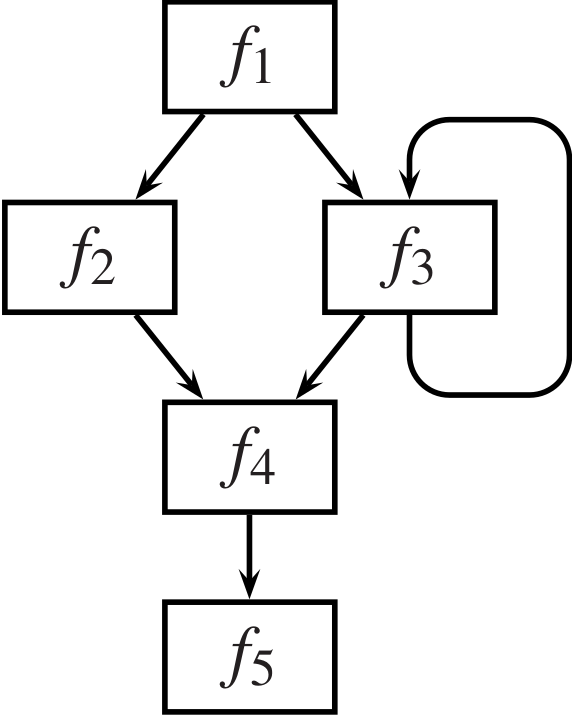
\includegraphics[scale=0.2]{functions_dataflow.png}
	  \label{fig:functions_dataflow}
	  \caption{Dataflow Flow Functions. One for each vertice of $G$. \citep{khedker2009data}}
  \end{subfigure}
  \begin{subfigure}[b]{0.40\textwidth}
	 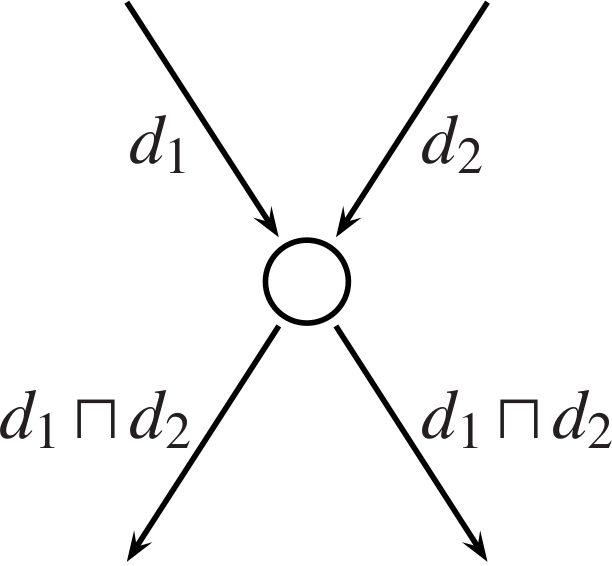
\includegraphics[scale=0.2]{meet_dataflow.png}
	  \label{fig:meet_dataflow}
	  \caption{Meet operation on a vertice, combining the generated information. \citep{khedker2009data}}
  \end{subfigure}
  \label{fig:dataflow}
\end{figure}

	Therefore, in abstract ways, we can define a dataflow framework instance as
	\begin{definition}
		An instance of dataflow framework is a 4-uple $(G, \mathcal{L}, \sqcap, \mathcal{F}_G)$,
		where
		\begin{itemize}
			\item $G = (V, E, s_0, F)$ is a Control-Flow Graph.
			\item $\mathcal{L}$ is a meet semitlattice satysfying the descending chain condition.
			\item $\bigsqcap$ is the meet operator of $\mathcal{L}$.
			\item $\mathcal{F}_G = \{f_1, f_2, \cdots, f_{|V|}\}$ is the set of monotonic transfer
			functions, one for each node $v \in V$, of the form of Equation (\ref{eq:foward}) or (\ref{eq:backward}).
		\end{itemize}
	\end{definition}

	

	\begin{subsubsection}{Liveness Analysis}
		One example of problem that can be solved with dataflow analysis is the \textit{liveness analysis},
		which is useful in the register selection phase. The purpose of this is to find, given a point
		in a CFGraph, if a certain variable will be used in the future. \cite{khedker2009data} defines the liveness analysis formaly as:
\begin{definition}
	Let $G = (V, E, s_0, F)$ be a CFGraph and $\mathbb{V}$ be the set of all variables
	of $G$. A variable $x \in \mathbb{V}$ is \textbf{live} at a program point $v \in V$
	if there exists a path from $v$ to $w \in F$ which contains a use of $x$ which is
	not preceeded by its definition.
\end{definition}

Therefore, a CGraph $G$, a dataflow framework instance for this would be:
$(G, \mathcal{L}, \bigsqcap, \mathcal{F}_G)$, where
\begin{itemize}
	\item $\mathcal{L} = (2^\mathbb{V}, \ssq)$, where $\mathbb{V}$ is the set of variables in the function represented by $G$.
	\item $\bigsqcap$ is the union operator $\bigcup$.
	\item $F_G = \conj{\texttt{in[} v \texttt{]}}{v \in V}$ where
	$\texttt{in[} v \texttt{]} = (\texttt{out[} v \texttt{]} - \texttt{kill[} v \texttt{]}) \cup \texttt{gen[} v \texttt{]}$.
\end{itemize}
which yields the dataflow equation:
\begin{equation}\label{eq:liveness}
\begin{split}
	\texttt{in[} v \texttt{]} &= (\texttt{out[} v \texttt{]} - \texttt{kill[} v \texttt{]}) \cup \texttt{gen[} v \texttt{]} \\
	\texttt{out[} v \texttt{]} &= 
	\begin{cases}
	  \emptyset,& \text{if } v \in F \\
	  \bigcup_{p \in \text{succ}(v)}\texttt{in[}p\texttt{]} ,& \text{otherwise} \\
	\end{cases}
\end{split}
\end{equation}

In this equation, $\texttt{gen[} v \texttt{]}$ represents the variables which turns
to be line at vertex $v$, and $\texttt{kill[} v \texttt{]}$ are the variables which
liveness are no longer valid at vertex $v$. For instance, consider the CFGraph
in Figure \ref{fig:cfg_liveness}. Here, we work on the set $\mathbb{V} = \{a, b, c, d\}$.
Solving Equation \ref{eq:liveness} using the propagation tecnique, simulated in Table
\ref{fig:table_cfg}. There, for instance, we can see that $d$ is not used anywhere
in the program because $d \not\in \ttt{out[}n_1\ttt{]}$.

\begin{figure}
\centering
	 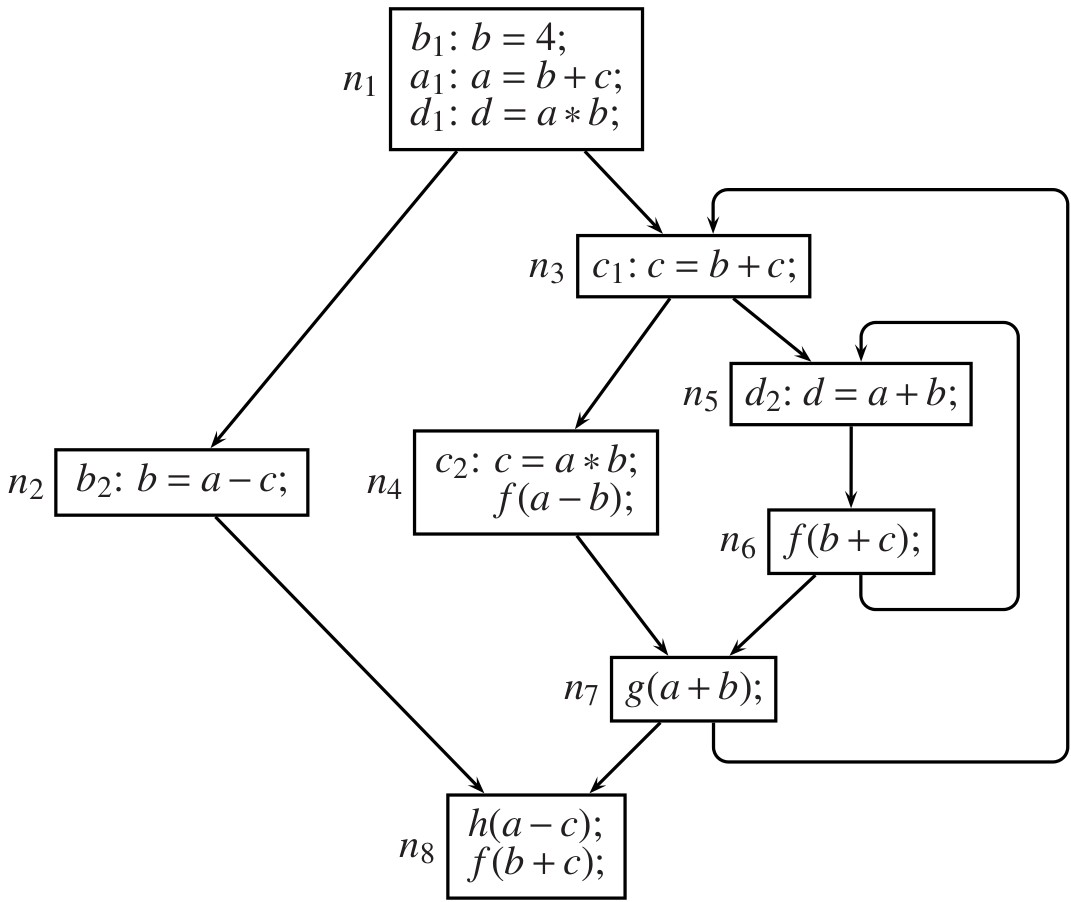
\includegraphics[scale=0.3]{cfg_liveness.png}
	  \caption{Example of CFGraph of a program function \citep{khedker2009data}.}
	  \label{fig:cfg_liveness}
\end{figure}

\begin{table}[]
\begin{tabular}{|c|c|c|c|c|c|c|}
\hline
\multirow{3}{*}{Vertex} & \multicolumn{2}{c|}{\multirow{2}{*}{Local Generation}}  & \multicolumn{4}{c|}{Global Information}                             \\ \cline{4-7} 
                        & \multicolumn{2}{c|}{}                                   & \multicolumn{2}{c|}{Iteration 1} & \multicolumn{2}{c|}{Iteration 2} \\ \cline{2-7} 
                        & $\texttt{gen[}n\ttt{]}$                        & $\ttt{kill[}n\ttt{]}$                   & $\ttt{out[}n\ttt{]}$             & $\ttt{in[} n\ttt{]}$             & $\ttt{out[}n\ttt{]}$             & $\ttt{in[} n\ttt{]}$            \\ \hline
$n_8$                   & $\{a, b, c\}$                & $\emptyset          $            & $\emptyset$               & $\{a, b, c\}$    & $\emptyset          $     & $\{a, b, c\}$    \\ \hline
$n_7$                   & $\{a, b\}$                   & $\emptyset          $            & $\{a, b, c\}$     & $\{a, b, c\}$    & $\{a, b, c\}$     & $\{a, b, c\}$    \\ \hline
$n_6$                   & $\{b, c\}$                   & $\emptyset          $            & $\{a, b, c\}$     & $\{a, b, c\}$    & $\{a, b, c\}$     & $\{a, b, c\}$    \\ \hline
$n_5$                   & $\{a, b\}$                   & $\{d\}      $            & $\{a, b, c\}$     & $\{a, b, c\}$    & $\{a, b, c\}$     & $\{a, b, c\}$    \\ \hline
$n_4$                   & $\{a, b\}$                   & $\{c\}      $            & $\{a, b, c\}$     & $\{a, b\}   $    & $\{a, b, c\}$     & $\{a, b\}   $    \\ \hline
$n_3$                   & $\{b, c\}$                   & $\{c\}      $            & $\{a, b, c\}$     & $\{a, b, c\}$    & $\{a, b, c\}$     & $\{a, b\}   $    \\ \hline
$n_2$                   & $\{a, c\}$                   & $\{b\}      $            & $\{a, b, c\}$     & $\{a, c\}   $    & $\{a, b, c\}$     & $\{a, c\}   $    \\ \hline
$n_1$                   & $\{c\}   $                   & $\{a, b, d\}$            & $\{a, b, c\}$     & $\{c\}      $    & $\{a, b, c\}$     & $\{c\}      $    \\ \hline

\end{tabular}
\caption{Solving the Equation \ref{eq:liveness} for Figure \ref{fig:cfg_liveness} 
\citep{khedker2009data}.}
\label{fig:table_cfg}
\end{table}

\end{subsubsection}

\end{subsection}

\begin{subsection}{Dominator Tree}
	One data structure used on optimization are
	\textit{dominator trees}. First we must define what \textit{domination} means:

	\begin{definition}
		Let $G = (V, E, s_0, F)$ be a Control-Flow Graph and $u, v \in V$. We say
		that $u$ \textbf{dominates} $v$ if every path from $s_0$ to $v$ go through
		$u$.
	\end{definition}

	That means that if some node $u$ dominates $v$, then it is certain that, in
	the current thread, the code in $u$ will be executed before $v$.
	\cite{georgiadis2006finding} presents a forward dataflow equation
	to compute the set of all dominators of a node:


\begin{equation}\label{eq:domtree_dataflow}
\begin{split}
	\texttt{dom[} v \texttt{]} &= 
	\begin{cases}
	  \{v\},& \text{if } v = s_0 \\
	  \left(\bigcap_{p \in \text{pred}(v)}\texttt{dom[}p\texttt{]}\right) \cup \{v\} ,& \text{otherwise} \\
	\end{cases}
\end{split}
\end{equation}

	However, instead of solving Equation \ref{eq:domtree_dataflow}
	every time we want to know if there is such dominance, or avoid
	holding a table containing \textit{every} dominator of a node,
	it is convenient to build a data structure that can quickly query
	such information. Such data structure is the \textit{dominator tree}
	of a CFGraph. Figure \ref{fig:domtree} presents the dominator tree of the CFGraph
	presented in Figure \ref{fig:cfg_liveness}.

\begin{figure}
\centering
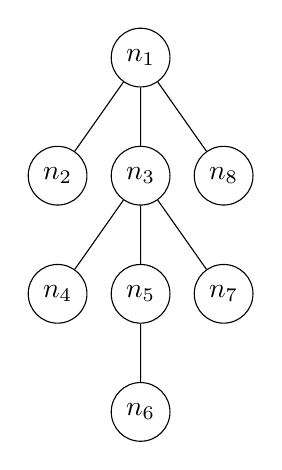
\begin{tikzpicture}[sibling distance=3em,
  every node/.style = {shape=circle,
    draw, align=center}]]
  \node {$n_1$}
    child { node {$n_2$} }
    child { node {$n_3$}
      child { node {$n_4$} }
      child { node {$n_5$}
        child { node {$n_6$} } }
      child { node {$n_7$} } }
  	child { node {$n_8$} };
\end{tikzpicture}
\caption{Dominator tree of Figure \ref{fig:cfg_liveness}}
\label{fig:domtree}
\end{figure}


	Dominator trees are often used to build the Static Single Form
	(SSA) of a CFGraph, and to detect loops in the Control-Flow
	Graph. \cite{appel2004modern} provides algorithms to detect
	loops using the CFGraph, which is useful when the language
	supports \texttt{goto}s. A faster algorithm
	(but complexier than the dataflow equation) algorithms to build
	the Dominator tree of a CFGraph is presented by
	\cite{georgiadis2006finding}.

\end{subsection}


\begin{subsection}{Static Single Assignment Form (SSA)}

Consider the following sequence of statements:
\begin{align}
x &= 2 \nonumber \\
y &= x \times x \nonumber \\
y &= y + 1 \nonumber \\
y &= 1 \nonumber
\end{align}

Clerly, the second and third statements can be discarded, and the first
and last statement can be discarded as well if there are no further use of $x$ and
$y$ in the program. However, how can the compiler know that? SSA form make
this clear. The idea is that variables can not be redefined, only new variables
can be created, which motivates the following defition.

\begin{definition}
	A program is in SSA form if there are at least one assignment for each
	variable.
\end{definition}

How can we represent the presented sequence of statement in this form then?
Create a new variable for each left-hand-side of the assignment

\begin{align}
x &= 2 \nonumber \\
y_1 &= x \times x \nonumber \\
y_2 &= y_1 + 1 \nonumber \\
y_3 &= 1 \nonumber
\end{align}

This will lead to the variable $y_2$ being unused because it is nowhere present
on the left-hand-side of any assignment, meaning that it can be discarded;
which will then imply that $y_1$ will be unused and can be discarded as well.

However, SSA form can get trickier to implement if there are jumps in the
programs, which is often the case with \texttt{if} and \texttt{while}
statements. In Figure \ref{fig:code_normal}, the value of \texttt{u}
depends upon which path the execution was taken, which depends on the
\textit{condition}. The solution fot this is to introduce a $\phi$
function, which will select the correct variable. Figure \ref{fig:code_ssa_form}
illustrates this.

\begin{figure}[ht]
    \centering
    \begin{subfigure}[b]{0.40\textwidth}

        \begin{lstlisting}[
            language=pseudocode,
            style=pseudocode,
            style=wider,
            functions={},
            specialidentifiers={extern, call},
            ]
            if (condition) then
                a = -1;
            else
                a = 1;
            end
            u = a*v;
        \end{lstlisting}
        \caption{\label{fig:code_normal}}
    \end{subfigure}
    \begin{subfigure}[b]{0.40\textwidth}
        \begin{lstlisting}[
                language=pseudocode,
                style=pseudocode,
                style=wider,
                functions={},
                specialidentifiers={extern, call, PHI},
              ]
            if (condition) then
                $a_1$ = -1;
            else
                $a_2$ = 1;
            end
            $a_3$ = $\phi$($a_1$, $a_2$)
            u = $a_3$*v;
        \end{lstlisting}
        \caption{\label{fig:code_ssa_form}}
\end{subfigure}
\caption{A program (a) and its SSA representation (b)}
\end{figure}

However, this illustration explains little about when to
place $\phi$ functions. A way of determine it is to use
the \textit{dominance frontier criteria}

\begin{definition}
	Let $G = (V, E, s_0, F)$ be a CFGraph and $u, v \in V$. We say that
	$u$ \textbf{strictly dominates} $v$ if $u$ dominates $v$, but
	$u \neq v$. We denote that $u$ idom $v$.
\end{definition}

\begin{definition}
	The \textbf{dominance frontier} of a node $x \in V$ is the set of all nodes $w \in V$
	such that $x$ dominates a predecessor of $w$, but does not strictly dominate $w$ \citep{appel2004modern}.
	Or, in set theory notation:
\end{definition}
\vspace*{-1cm}
	$$\texttt{dfront[}x\texttt{]} = \conj{w \in V}{x \text{ dom } y \text{ for some } y \in \text{pred}(w) \text{ and } y \text{ does not sdom } w}$$

This definition looks blury, but it can be easily understeand as the
\textit{border of nodes where the dominance stops}.  Figure \ref{fig:dom_frontier} illustrates this
concept with a plot of the dominated nodes of $v_5$ in the beige area, and the dominance frontier
in the green area.

\begin{figure}[ht]
 \centering
 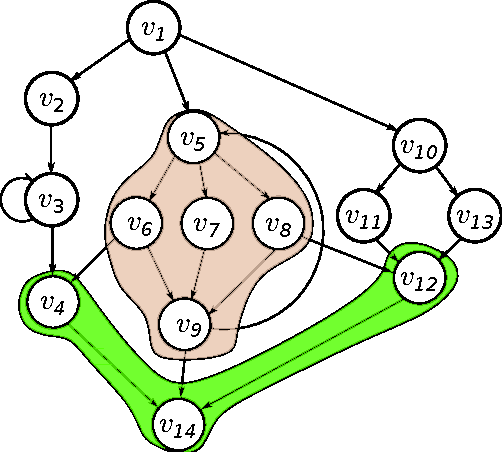
\includegraphics[scale=1.0]{dom_frontier.pdf}
 \caption{Dominance frontier of node $v_5$. Beige is dominated by $v_5$. Green is in dominance frontier of $v5$.}
 \label{fig:dom_frontier}
\end{figure}

The criteria to place $\phi$-functions are the following: When a node $x$ contains a defintion
of a variable $a$, then any node $z$ in the dominance frontier of $x$ needs a $\phi$ function
for $a$ \cite{appel2004modern}.

\end{subsection}

\begin{section}{Callgraphs and Inter-Procedural Analysis}

Some optimizations requires interaction with other functions, one clear example
of this are \textit{function inlining}. When there is a function call, the
call itself consumes time, and therefore it may be interesting to copy and
paste the content of the function being called and remove the call at all.
Therefore, a data structure is required to model the interactions between
functions.

That is the purpose of a \textit{callgraph}: each vertex denotes a function,
and each edge represents a call between two functions. 

\begin{definition}
	A callgraph is a graph $G = (V, E)$, where $V = \{f_1, f_2, \cdots, f_{|V|}\}$
	are the set of functions, and $E = \conj{(u, v)}{u, v \in V}$ are the set
	of edges representing a function call. Given $e = (u, v) \in E$, this means
	that $u$ calls $v$. $u$ is the caller function, and $v$ is the callee function.
\end{definition}

Figure \ref{fig:call_graph} gives an example of a callgraph. When applying
Inter-Procedural Optimizations, each vertex can also hold some sort of
\textit{summary} of the function instead the entire function, because often
the program being compiled is large enough that there is not enough memory
to hold the contents of the functions. This is the case when working with
the Link Time Optimization technique.

There are some extenstions to the dataflow frameworks to work on Inter-Procedural
Optimizations \citep{khedker2009data}, however their require complete information
about the function in memory, which may not be present in this stage on compilers
such as GCC \citep{gcc_ipa}.

\begin{figure}[ht]
\centering
  \begin{subfigure}[b]{0.40\textwidth}
      \begin{lstlisting}[
        language=pseudocode,
        style=pseudocode,
        style=wider,
        functions={},
        specialidentifiers={extern, call},
      ]
        extern function g,h

        function f()
            call $g$
            call $h$
        end

        function main()
            call $f$
            call $h$
        end
      \end{lstlisting}
  \end{subfigure}
  \begin{subfigure}[b]{0.40\textwidth}
    \tikzstyle{line} = [draw, -latex]
    \tikzstyle{node} = [draw, circle]
    \begin{center}
    \scalebox{1.0}{
    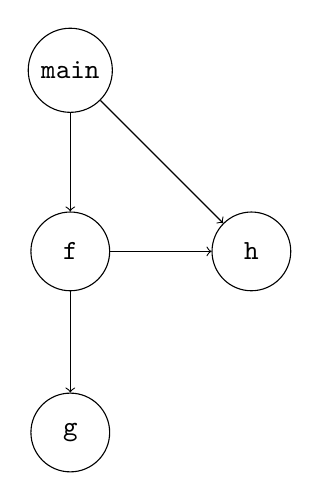
\begin{tikzpicture}[node distance = 2.3cm, minimum height = 1cm, auto]
        % Place nodes
        \node [node]                    (main) {\texttt{main}};
        \node [node, below of = main]        (f) {\texttt{f}};
        \node [node, below of = f]           (g) {\texttt{g}};
        \node [node, right of = f]           (h) {\texttt{h}};

        % Draw edges
        \draw[->]    (main)           -- (f);
        \draw[->]    (f)              -- (g);
        \draw[->]    (f)              -- (h);
        \draw[->]    (main)           -- (h);
    \end{tikzpicture}
    }
    \end{center}
  \end{subfigure}
  \caption{Um programa e seu respectivo grafo de chamada de funções}
  \label{fig:call_graph}
\end{figure}

\begin{subsection}


\end{subsection}

\end{section}

\end{section}

\begin{section}{Software Engineering in Compilers}

%Para evitar confusões a respeito das diferentes linguagens que um compilador
%trabalha em seus muitos estágios, é adotado a seguinte nomenclatura neste trabalho:
%Denote \textit{Linguagem Fonte} como sendo a linguagem
%na qual o código fonte do programa a ser compilado foi originalmente escrito;
%\textit{Linguagem Intermediária} uma das linguagens internas do compilador; e
%\textit{Linguagem Alvo} a linguagem na qual o compilador deverá gerar código.

To avoid confusion regarding the various languages that the compiler works on,
we denote the following definitions on this work: Denote \textit{Source
Language}, as the language in which the code being compiled was originally
written; \textit{Intermediary Language} as the languages used internally in the
compiler; and \textit{Target Language} the language in which the compiler must
generate the code.

Compilers are large projects destined for the translation of source code
between distinct programming languages. Usually, compilers translate high-level
languages such as C, to assembly language. However, this is not a rule once
there exist compilers designed for the translation between high-level language.
Such compilers are called a Transpilator.

%Compiladores são grandes projetos destinados a tradução de códigos fonte
%entre distintas linguagens de programação. Normalmente, compiladores traduzem
%linguagens de alto nível, como C, para linguagens mais próximas da máquina,
%como a linguagem de montagem - embora isso não seja uma regra pois existem
%compiladores cuja única tarefa é realizar uma tradução entre duas linguagens
%de alto nível.

%Compiladores também costumam otimizar
%o código que passam por eles, aplicando diversas heurísticas de
%maneira a acelerar o código a ser produzido, substituindo trechos de código por
%outros mais eficientes, reordenando as instruções do programa, etc.

Compilers also usually optimize the code that passes in them, applying several
heurístics and algorithms to produce faster code, replacing pieces of code with
more efficient ones, reordering program instructions, aligning the code in
caches, etc.

Being a large program, there is a great interest in avoiding rewriting a
compiler when a new language is proposed, or when new hardware is created. For
that, compiler writers usually adopt the following modularization
\citep{redhat} \citep{llvm}, as illustrated by Figure \ref{fig:compiler_arch}:

%Por serem programas extremamente grandes, existe um grande interesse em evitar
%reescrever um novo compilador
%sempre que uma nova linguagem é proposta, ou um novo \textit{hardware} é criado.
%Para isso, a seguinte modularização é largamente adotada por projetistas de
%compiladores \citep{redhat} \citep{llvm}, conforme ilustrado na Figura \ref{fig:compiler_arch}:
%

\begin{itemize}

\item A Front End for each Source Language. In this module are executed the
lexical and syntactical analysis to construct the Abstract Syntax Tree (AST).
Following that, this structure is converted to another compiler's IR.

\item A Middle End, responsible for applying several hardware-independent
optimizations to the already converted IR code.

\item A Back End for each Target Language, responsible to translate the IR to
the Target Language. Here, hardware-dependent optimizations are employed, such
as register allocation and instruction selection.

\end{itemize}

%\begin{itemize}
%    \item Um \textit{Front End} para cada Linguagem Fonte.
%	Neste módulo são executadas as análises léxica e sintática, com a
%        finalidade de construir uma Árvore de Sintaxe Abstrata (AST), para que em
%seguida, ela seja convertida para uma Linguagem Intermediária do compilador.
%
%    \item Um \textit{Middle End}, responsável por aplicar diversas otimizações
%independentes de arquitetura no código já convertido para a Linguagem Intermediária.
%
%    \item Um \textit{Back End} para cada linguagem alvo, responsável por converter a linguagem intermediária
%na linguagem alvo. Aqui outras otimizações específicas da linguagem alvo são realizadas,
%como alocação de registradores e seleção de instruções.
%\end{itemize}

However, this modularization is completely optional: older compilers destined
to simply doing a direct translation between languages, such as the UNIX C
Compiler, do not have an IR \citep{ritchie1979tour}. Not only that, several
textbooks about compilers do not mention the Middle-End part, being a part of
the Beck-End of the compiler \citep{dragonbook}. Not adopting this
modularization simplifies the project, but also complicates the insertion of
new programming languages, as well as adding support to new hardware.

%Porém, essa modularização é opcional: compiladores mais antigos destinados a fazer uma
%conversão direta entre duas linguagens, como o UNIX C Compiler, não costumam usar uma linguagem
%intermediária \citep{ritchie1979tour}, além de diversos livros-texto não mencionarem tal módulo, fundindo suas
%funcionalidades com o \textit{Back End} \citep{dragonbook}. Não adotar tal metodologia
%simplifica o projeto, mas dificulta a inserção de suporte a novas
%linguagens de programação.


\begin{figure}
\tikzstyle{block} = [rectangle, draw, fill=white,
    text width=6em, text centered, rounded corners, node distance=5cm, auto, minimum height=2em]
\tikzstyle{line} = [draw, -latex]
\tikzstyle{cloud} = [draw, ellipse,fill=white, node distance=2cm,
    minimum height=2em]

\begin{center}
\scalebox{0.8}{
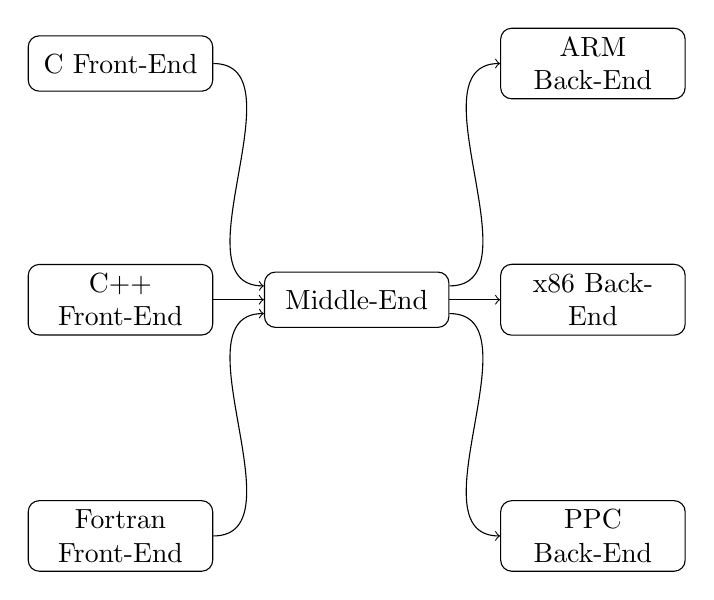
\begin{tikzpicture}[node distance = 3cm, auto]
    % Place nodes
    \node [block]                      (front_c)    {C Front-End};
    \node [block, below of=front_c]    (front_cpp)  {C++ Front-End};
    \node [block, below of=front_cpp]  (front_fort) {Fortran Front-End};
    \node [block, right of=front_cpp]  (middle)     {Middle-End};
    \node [block, right of=middle]     (back_x86)   {x86 Back-End};
    \node [block, above of=back_x86]   (back_arm)   {ARM Back-End};
    \node [block, below of=back_x86]   (back_ppc)   {PPC Back-End};


    \coordinate [left of=front_c]    (c_code);
    \coordinate [left of=front_cpp]  (cpp_code);
    \coordinate [left of=front_fort]  (fort_code);

    \coordinate [right of=back_x86] (x86_code);
    \coordinate [right of=back_arm] (arm_code);
    \coordinate [right of=back_ppc] (ppc_code);

    % Draw edges
    \draw[->]    (front_c.east)     to [out=0,in=180] ([yshift=0.5em]  middle.west);
    \draw[->]    (front_cpp.east)   to [out=0,in=180] (middle.west);
    \draw[->]    (front_fort.east)  to [out=0,in=180] ([yshift=-0.5em] middle.west);

    \draw[->]    ([yshift=-0.5em] middle.east)  to [out=0,in=180] (back_ppc.west);
    \draw[->]    (middle.east)                  to [out=0,in=180] (back_x86.west);
    \draw[->]    ([yshift=0.5em] middle.east)   to [out=0,in=180] (back_arm.west);

    %\draw[->]    (sintatico.west)   -- (lexico.east)    node[midway] {próximo\_token()};
    %\draw[->]    (fonte.west)       -- (lexico.west)    node[pos=0, above] {Código Fonte};
    %\draw[->]    (sintatico.east)   -- (ast.west)       node[pos=1, above] {Árvore Abstrata};
\end{tikzpicture}
}
\end{center}

\caption{Compiler Architecture}
\label{fig:compiler_arch}
\end{figure}

%\begin{subsection}{\textit{Front-End}}
\begin{subsection}{Front-End}

A Front-End is a module responsible for direct interaction with the code
written in the Source Language, which means from a Software Engineering
perspective, for adding support to a new Source Language, it is enough to write
a new Front-End. It is also possible that some classes are shared between
frontends, which may be the case of a compiler that supports both C and C++.

%Um \textit{Front End} é um módulo responsável por interagir diretamente com o
%código escrito na Linguagem Fonte a ser compilado. Ele costuma ser único
%para cada Linguagem Fonte, ou seja, para inserir suporte a uma nova
%Linguagem Fonte, basta implementar um novo \textit{Front End}, mas é
%possível que algumas classes sejam
%compartilhadas, como no caso de um compilador que dê tanto para C quanto para e C++.


As a first step, the Front-End performs a lexical and syntactical analysis for
generating an AST and verify if the input text belongs to the language. It is
also responsible for printing parsing errors in a way that the user can easily
understand them. The Front-End also populates the Symbol Table of the compiler
with symbols that it has seen so far when compiling the program for checking if
there are references to undefined symbols. These three pieces (the Lexical
Analyser, the Syntactic Analyser, and the Symbol Table) frequently communicate
with each other, as illustrated in Figure \ref{fig:lexico_sintatico}.

%Como primeiro passo, \textit {Front End} realiza uma análise
%léxica e sintática, com a finalidade de gerar uma AST e verificar
%se o texto dado como entrada realmente pertence à linguagem.
%Estes dois analisadores se comunicam constantemente, conforme ilustrado na Figura
%\ref{fig:lexico_sintatico}.

\begin{figure}
\tikzstyle{block} = [rectangle, draw, fill=white,
    text width=6em, text centered, rounded corners, node distance=9cm, auto, minimum height=2em]
\tikzstyle{line} = [draw, -latex]
\tikzstyle{cloud} = [draw, ellipse,fill=white, node distance=2cm,
    minimum height=2em]

%TODO: Adcionar a tabela de símbolos aqui.
\begin{center}
\scalebox{0.8}{
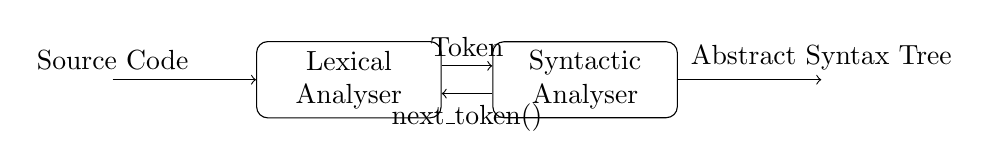
\begin{tikzpicture}[node distance = 3cm, auto]
    % Place nodes
    \node [block]                    (lexico) {Lexical Analyser};
    \node [block, right of = lexico] (sintatico) {Syntactic Analyser};
    \coordinate [left of=lexico]     (fonte);
    \coordinate [right of=sintatico] (ast);

    % Draw edges
    \draw[->]    ([yshift=0.5em] lexico.east)       -- ([yshift=0.5em] sintatico.west) node[midway] {Token};
    \draw[->]    ([yshift=-0.5em] sintatico.west)   -- ([yshift=-0.5em] lexico.east)    node[midway] {next\_token()};
    \draw[->]    (fonte.west)                       -- (lexico.west)    node[pos=0, above] {Source Code};
    \draw[->]    (sintatico.east)                   -- (ast.west)   node[pos=1, above] {Abstract Syntax Tree};
\end{tikzpicture}
}
\end{center}

\caption{Interactions between the Lexical, Syntactic Analyser and the Symbol Table}
\label{fig:lexico_sintatico}
\end{figure}

%    Primeiro, a análise léxica é responsável por ler o arquivo
%de texto contendo o código fonte, e quebrar as palavras em \textit{tokens}, que
%serão alimentados para o analisador sintático. Por consequência, ele é capaz de
%realizar alguns filtros, \textit{e.g}. ignorar os comentários, identificar constantes
%numéricas, eliminar espaços desnecessários, e substituir um \textit{token} por
%outro.
%Analisadores léxicos também podem ser usados para substituição
%de macros, como implementado pelo preprocessador do C
%(CPP)\footnote{https://gcc.gnu.org/onlinedocs/cppinternals/Lexer.html}.

First, the Lexical Analyser is responsible for reading a text file containing
the Souce Code and splitting the words in the file in Tokens. As a consequence,
it is capable of applying some filters, e.g. ignore commentaries, identify
numerical constants, remove unnecessary spaces, and replace a token with
another.  Lexical Analysers can also be used for macro expansion, as
implemented in the C preprocessor
(CPP)\footnote{https://gcc.gnu.org/onlinedocs/cppinternals/Lexer.html}.

%Geralmente, os Analisadores Léxicos são implementados utilizando autômatos
%por diversos motivos, entre eles sua atrativa complexidade computacional
%$O(n)$, onde $n$ é o tamanho da entrada, pela existência de algoritmos
%para converter expressões regulares em autômatos \citep{thompson}, e pela
%existência de algoritmos para minimização de estados de um autômato
%\citep{hopcroft1971n}. Isto possibilita que geradores de analisadores léxicos
%como o \texttt{Flex}\footnote{https://www.gnu.org/software/flex/}
%sejam bastante eficientes.

Usually, Lexical Analysers are implemented using $\DFA$, in which each
acceptance state corresponds to a generated token. This yields a fast,
$O(n)$ algorithm for detecting tokens in the code, which will be feeded
to the Lexical Analyser. There are even Lexical Analyser Generators such
as \textit{Flex}\footnote{https://www.gnu.org/software/flex/}, which
are extremelly efficient.

Together with the Lexical Analyser, a Syntactic Analyzer is responsible to
generate an Abstract Syntax Tree (AST), inspecting the sequence of tokens
provided by the Lexical Analyser, or point out why the input string is
not valid. The objective of a Syntatic Analyser is to construct
an Abstract Syntax Tree (AST) by keeping track of the reduction decisions
(in the case of the Botton-Up parser such as $\LR{1}$) or the derivation
decisions (which is the case of a Top-Down parser such as Recursive-Descent)
of the input string. The decision of doing type analysis, checking for
undefined usage of variables, etc, can be done while building this
AST, or postergated to a next stage, called the Semantic Analysis,
which is still part of the Front-End.

After the AST is generated and the Semantic Analsysis are completed, it is
often converted to an Intermediate Representation (IR), where Target-Independent
Optimizations are performed. This yields the control to the Middle-End of
the compiler.

\end{subsection}

\begin{subsection}{Middle End}

The Middle-End is responsible to work on one or more Intermediate Representations
(IR) of the compiler. If there are checks which can be postponed in the Front-End
to this stage, it is preferible, once it avoids these checks on every Source
Langue's Front-End.

There are several representations for a IR, however, we will focus on those
used in GIMPLE to avoid extending this text unecessary.

Existem várias representações convenientes para a Linguagem Intermediária,
mas destaca-se para fins de otimização
a \textit{Three-Address Code}, que normalmente é usada em conjunto com
a \textit{Static Single Assignment} (SSA).


\begin{subsubsection}{Otimizações Independente de Arquitetura}

Uma das funcionalidades mais atrativas de um compilador é sua
capacidade de fazer otimizações no código enquanto mantém
a corretude do mesmo, principalmente quando
o alvo é uma linguagem de montagem. Um compilador com essa
funcionalidade é capaz de gerar código que economiza energia
gasta em processamento, poupa esforços de otimização, desenvolvimento,
entre outros.

Considerando o contexto de um compilador capaz de compilar
diversas linguagens para os mais variados alvos, o \textit{Middle End} é
exatamente onde maior parte do tempo gasto na implementação de otimizações é
alocado, pois isto implica gerar um código mais eficiente para todas as
Linguagens Alvo cujo o compilador dá suporte.

Como o \textit{Front End} já traduziu todo o código para a linguagem
intermediária, então é perfeitamente possível marcar o início de
todas as funções do código. Com isto, é possível particionar o
conjunto das possíveis otimizações em dois conjuntos disjuntos:

\begin{itemize}
    \item Otimizações \textit{Intra-Procedurais}: Otimizam cada função sem
interagir com as demais funções do programa.

    \item Otimizações \textit{Inter-Procedurais}: Procuram observar o programa
como um todo, observando as interações de cada função com as demais
funções do programa. Um exemplo clássico é remover funções não utilizadas, e
decidir se uma determinada função será compilada com o atributo \texttt{inline}.
\end{itemize}
Essa distinção é útil pois não há dependência entre as funções
ao aplicar uma otimização \textit{Intra-Procedural}, e portanto as
funções podem ser processadas em paralelo.
Diversas otimizações
clássicas como Invariante de Laços, Propagação de Constantes,
Eliminação de Redundância, Eliminação de Subexpressão Comum,
Propagação de Constantes e Eliminação de Código Morto são
classificadas como tal, reforçando o argumento de paralelização.

Entretanto, esse argumento não é válido para as otimizações \textit{Inter-Procedurais}, pela
própria definição. Estas otimizações são normalmente aplicadas
utilizando algoritmos em grafos:
Cada rotina é representado como um vértice, e existe um arco de $f$
à $g$ se $f$ chama $g$ em seu corpo, conforme ilustrado na Figura
\ref{fig:call_graph}. Construir tal grafo pode ser
um desafio dependendo da linguagem de programação, principalmente
quando se utiliza orientação a objetos devido a possibilidade de
sobrescrita de métodos. Por fim, mais detalhes a respeito dos
algoritmos referentes a essas otimizações são discutidos por
\cite{khedker2009data}.

\begin{figure}[ht]
\centering
  \begin{subfigure}[b]{0.40\textwidth}
      \begin{lstlisting}[
        language=pseudocode,
        style=pseudocode,
        style=wider,
        functions={},
        specialidentifiers={extern, call},
      ]
        extern function g,h

        function f()
            call $g$
            call $h$
        end

        function main()
            call $f$
            call $h$
        end
      \end{lstlisting}
  \end{subfigure}
  \begin{subfigure}[b]{0.40\textwidth}
    \tikzstyle{line} = [draw, -latex]
    \tikzstyle{node} = [draw, circle]
    \begin{center}
    \scalebox{1.0}{
    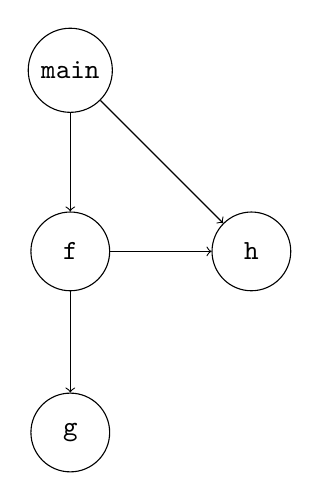
\begin{tikzpicture}[node distance = 2.3cm, minimum height = 1cm, auto]
        % Place nodes
        \node [node]                    (main) {\texttt{main}};
        \node [node, below of = main]        (f) {\texttt{f}};
        \node [node, below of = f]           (g) {\texttt{g}};
        \node [node, right of = f]           (h) {\texttt{h}};

        % Draw edges
        \draw[->]    (main)           -- (f);
        \draw[->]    (f)              -- (g);
        \draw[->]    (f)              -- (h);
        \draw[->]    (main)           -- (h);
    \end{tikzpicture}
    }
    \end{center}
  \end{subfigure}
  \caption{Um programa e seu respectivo grafo de chamada de funções}
  \label{fig:call_graph}
\end{figure}
    Após todo esse processo de otimização, o código nesta linguagem ainda
pode sofrer transformações para outras Linguagens
Intermediárias para algo que seja mais próximo do
\textit{hardware}-alvo (nos casos em que a compilação tem como alvo código de máquina).
Finalmente, após essa sequência de transformações, o controle é
passado ao \textit{Back End} do compilador, onde ele será transformado na
Linguagem Alvo.

\end{subsubsection}

\end{subsection}

\begin{subsection}{\textit{Back End}}
    O \textit{Back End} é responsável pela geração do código final na
Linguagem Alvo, além otimizações dependentes da arquitetura. Sendo assim,
ele também deve efetuar otimizações referentes
a seleção de instruções mais eficazes e alocação registradores
da melhor maneira possível para as variáveis do programa, caso a linguagem alvo
seja a Linguagem de Montagem.

    Existem diversas técnicas para selecionar instruções. Uma estratégia possível
é substituição de macros, onde as instruções são substituídas
observando localmente cada linha de código da Linguagem Intermediária. Esta estratégia
tem a vantagem de realizar uma tradução rápida e de fácil implementação, mas que gera
código ineficiente, conforme ilustrado na Figura \ref{fig:macro_exp}. Existem otimizações
que podem ser aplicadas para melhorar o resultado das instruções geradas, sendo a mais famosa
delas a \textit{Peephole Optimization}, que tenta remover leituras e escritas desnecessárias
a memória buscando instruções que se anulam.

\begin{figure}
\tikzstyle{block} = [rectangle, draw, fill=white,
    text width=15em, text centered, rounded corners, node distance = 1cm and 1cm, auto, minimum height=2em]
\tikzstyle{line} = [draw, -latex]
\tikzstyle{cloud} = [draw, ellipse,fill=white, node distance=2cm,
    minimum height=2em]

\begin{center}
\scalebox{0.8}{
\begin{tikzpicture}
    % Place nodes
    \begin{scope}[node distance = 1cm and 5cm]
    \node [block]                  (c1) {$\textit{fib}_i = \textit{fib}_{i-1} + \textit{fib}_{i-2}$};
    \node [block, below=of c1]     (c2) {$\textit{fib}_{i-2} = \textit{fib}_{i-1}$};
    \node [block, below=of c2]     (c3) {$\textit{fib}_{i-1} = \textit{fib}_{i}$};
    \end{scope}

    \node [block, right=of c1]     (asm1) {\texttt{mov eax, DWORD [ebp-8]} \\ \texttt{mov ebx, DWORD [ebp-12]} \\ \texttt{add eax, ebx} \\ \texttt{mov [ebp-4], eax}  };
    \node [block, right=of c2]     (asm2) {\texttt{mov eax, DWORD [ebp-8]} \\ \texttt{mov [ebp-12], eax}};
    \node [block, right=of c3]     (asm3) {\texttt{mov eax, DWORD [ebp-4]} \\ \texttt{mov [ebp-8], eax}};

    % Draw edges
    \draw[->]    (c1.east)        -- (asm1.west);
    \draw[->]    (c2.east)        -- (asm2.west);
    \draw[->]    (c3.east)        -- (asm3.west);
\end{tikzpicture}
}
\end{center}

\caption{Seleção de instruções usando expansão de macros para i386. Sintaxe da Intel.}
\label{fig:macro_exp}
\end{figure}

Uma outra maneira é realizar a seleção de instruções através de uma
representação em árvore da Linguagem Intermediária.  Inicialmente
desenvolvida como um aperfeiçoamento da técnica de substituição de macros,
essa técnica busca por padrões na árvore e as substitui pelas instruções de
acordo com uma regra especificada.  As primeiras implementações deste
método eram heurísticas simples, substituindo os padrões conforme eles eram
encontrados, sem se preocupar em escolher o melhor conjunto de padrões.

\cite{glanville1978} evoluiu tal método utilizando as mesmas técnicas de
análise léxica e sintática normalmente empregadas no \textit{Front End}. A
partir do algoritmo LR(1), Graham conseguiu postergar a emissão de código
utilizando a máquina de estados desse algoritmo para armazenar um contexto
limitado das instruções já vistas. Quando o algoritmo decide emitir código,
é selecionado o conjunto de instruções que minimiza o custo total do
contexto atual. Isso permite selecionar instruções em tempo linearmente
proporcional ao tamanho da expressão e considerar o custo das instruções no
momento de emitir o código.

Embora a técnica de Graham-Glanville tenha uma complexidade computacional bem
atraente, esse método se mostrou difícil de implementar na prática devido a
quantidade de instruções disponíveis nos processadores, resultando em uma
máquina de estados com milhares de estados, e vários conflitos de ambiguidade.
Também é importante notar que esse método não é capaz de gerar código com custo
ótimo no caso geral, pois uma vez que o algoritmo decide emitir as instruções,
elas não serão mais modificadas independentemente das instruções lidas
posteriormente \citep{blindell2016instruction}.

Ainda considerando a seleção de instruções em uma representação em árvore,
é possível selecionar as instruções de maneira ótima através de Programação
Dinâmica, conforme proposto por \cite{ripken1977formale}.  A ideia consiste em
observar que para minimizar o custo de selecionar os padrões na árvore inteira,
basta considerar o melhor custo dos filhos
e tentar selecionar um padrão que minimiza o custo da raiz. Matematicamente, seja
$P_n$ o conjunto de padrões que são possíveis de aplicar em $n$, o nó atual da árvore.
Então o custo mínimo $DP[n]$ é:
\[
    DP[n] =
     \begin{cases}
       \min_{p \in P_n} CUSTO[p]  &\quad\text{se } n \text{ é nó folha.}\\
       \min_{p \in P_n} CUSTO[p] + \sum_{f \in FILHO[p]} DP[f] &\quad\text{ caso contrário.}\\
     \end{cases}
\]

Outra maneira de selecionar instruções é através de uma representação em 
Grafos Acíclicos Direcionados (DAGs). Sua vantagem é a possibilidade de representar
subexpressões em comum em uma expressão, mas infelizmente selecionar instruções
de maneira ótima em um DAG é NP-completo \citep{koes2008near}.  A maioria das
técnicas empregadas em seleção de instruções utilizando DAGs são gulosas, como
o caso do \cite{llvm_insn_selection}.

Por fim, uma discussão mais detalhada sobre
as técnicas de geração de código de máquina é discutida por
\cite{blindell2016instruction}. Além disso, para
adicionar suporte a uma nova arquitetura ou linguagem
alvo, basta implementar um novo \textit{Back End}, aproveitando todo
o código já implementado nas etapas anteriores.

\end{subsection}


\end{section}


\begin{section}{O Compilador GCC}

A coleção de compiladores da GNU, também conhecido como GCC, é um projeto
iniciado por Richard Stallman com a primeira versão disponibilizada ao público
em Março de 1987. Tal versão apenas fornecia suporte a linguagem C, mas já permitia
    gerar código para diversas arquiteturas \citep{gcc_first_ver}.
Hoje, o GCC fornece suporte a diversas Linguagens Fonte como C, C++, Fortran, Go, Ada,
e várias arquiteturas, como i386, amd64, riscv, arm, ppc, pdp-11. O GCC também
é um compilador otimizador, ou seja, ele é capaz de alterar o código fornecido
pelo usuário com a finalidade de gerar código mais eficiente, sem alterar a semântica do programa. Isso é
possível por conta das várias Linguagens Intermediárias implementadas no
GCC: GENERIC, GIMPLE, e RTL. O compilador executa vários
passos de otimização em cada uma dessas linguagens intermediárias.

\begin{subsection}{GENERIC}

    O GENERIC é uma linguagem intermediária que possibilita representar quaisquer
funções do programa através de árvores. Tal linguagem é um superconjunto
das funcionalidades e atributos que cada Linguagem Fonte contém, por exemplo, atributos
como \texttt{volatile} de C e C++ contém uma representação nessa linguagem.
Outras funcionalidades são: chamadas de função, declaração de variáveis, classes,
funções, expressões, entre outros \citep{generic}.

    Essa linguagem contém uma representação mais próxima de como o programa foi
escrito pelo programador, ou seja, não são feitas modificações nas expressões.
Sendo assim, essa linguagem
intermediária não se enquadra nas categorias de \textit{Three Address Code},
ou \textit{Static Single Assignment} pois isso demanda modificações no código.
O objetivo principal dessa linguagem
é facilitar a tradução para a próxima linguagem intermediária, a GIMPLE, e assim
facilitar o desenvolvimento dos \textit{Front End} do compilador, mas isso não
significa que otimizações não possam ser aplicadas aqui.

    O GCC possui um mecanismo de substituição de nós em sua representação
interna, dando suporte a árvore construída em GENERIC. Esse mecanismo é simples: o
compilador procura por uma cadeia de nós na árvore, buscando padrões,
como especificado no arquivo \texttt{gcc/match.pd}, e os substitui pelo o que
foi instruído na regra de substituição. Esse mecanismo, embora simples, permite
com que diversas simplificações matemáticas sejam implementadas no código, o
que pode significar uma melhora de até $10\times$ em casos particulares
\citep{sinatan}.

    Por fim, cada \textit{Front End} do GCC é responsável por traduzir o
código fonte para esta linguagem intermediária. Para visualizar um programa
nessa representação, basta compilá-lo utilizando o atributo
\texttt{-fdump-tree-original}.

\end{subsection}

\begin{subsection}{GIMPLE}

O GIMPLE é outra linguagem intermediária do GCC, basicamente consistindo na
conversão de GENERIC para \textit{Three Address Code}, havendo ainda um passo
posterior adicionando uma representação SSA a esta linguagem. Assim como o
GENERIC, a GIMPLE também é geral o suficiente para representar os atributos
de todas as Linguagens Fonte de cada \textit{Front End}.  Essa linguagem
intermediaria é baseada na linguagem SIMPLE, do compilador McCAT \citep{gimple}.

    Por ser uma linguagem do tipo \textit{Three Address Code}, é aqui onde
grande parte das otimizações livre de arquitetura são aplicadas, e portanto o
GIMPLE fornece uma \textit{Application Programming Interface} (API) detalhada
para efetuar alterações no código, incluindo a representação em forma SSA para análise
de fluxo que os passos de otimização deverão utilizar.

    Por fim, o compilador pode ser instruído a escrever o código em
GIMPLE através da opção \texttt{-fdump-tree-gimple}, ou então usando
a opção \texttt{-fdump-tree-ssa} para escrever a representação SSA
em disco.

\end{subsection}

\begin{subsection}{\textit{Register Transfer Language}}

    Por fim, a última linguagem intermediária do compilador GCC é a
\textit{Register Transfer Language} (RTL). A sintaxe dessa linguagem
tem inspiração no Lisp, onde as expressões são representadas por uma
lista de comandos \citep{rtl}.

    A RTL é uma linguagem que visa ser extremamente próxima da linguagem
de montagem, mas ainda sendo genérica o suficiente a ponto de ser compatível
com todas as Linguagens Alvo do GCC.
Para isso, ela representa uma máquina com infinitos
registradores, que serão alocados em registradores reais no passo correspondente.
Caso a arquitetura alvo não tenha o número necessário de
registradores, as variáveis deverão ser guardadas em memória. Por exemplo,
no caso do i386, elas deverão ser salvas na pilha. Esse processo é conhecido
como \textit{Register Spilling}.

    Essa é a última Linguagem Indermediária antes da geração do código final. O
\textit{Back end} transformará o código nessa linguagem para a Linguagem Alvo
substituindo uma sequência de instruções em RTL por uma sequência de instruções
na Linguagem Alvo. Essa escolha segue um sistema
de custos no qual o compilador procura escolher uma sequência de instruções
que minimiza a soma do custo total da tradução.

    Na arquitetura i386, as regras de substituição estão implementadas
em \texttt{gcc/config/i386/i386.md}, com o sistema de custos definido
na \texttt{struct processor\_costs}, no arquivo \texttt{gcc/config/i386/i386.h}.
Cada processador da arquitetura i386 deve definir o custo de cada instrução,
como definido em \texttt{gcc/config/i386/x86-tune-costs.h}.


\end{subsection}

\begin{subsection}{Passos de Otimização}
    O GCC possui vários passos de otimização que são aplicados em cada linguagem
intermediária. Esses passos são divididos em três etapas:

    \begin{enumerate}
        \item \textbf{IPA} - Após a tradução do programa para GENERIC, o
            compilador constrói um grafo de chamadas de função. Para cada
            chamada de $g$ a partir de $f$, é inserido um arco de $f$ à $g$.
            Com isso o compilador pode decidir eliminar funções que não são
            utilizadas no programa simplesmente descartando a função do
            código, ou então decidir que uma função precisa ser convertida para
            \texttt{inline}, como programado em \texttt{pass\_ipa\_inline}.

        \item \textbf{GIMPLE} - Após a etapa IPA, são executados os passos
            de otimização do GIMPLE. Tais passos são executados em cada
            função de maneira independente, ou seja, são otimizações
            Intra Procedurais.
            Existem diversas otimizações que são aplicadas nesse passo.
            Por exemplo, aqui é aplicado a \texttt{pass\_vectorize},
            que tenta vetorizar um laço, a \texttt{pass\_parallelize\_loops},
            que tenta fazer paralelização automática de laços, a
            \texttt{pass\_sincos}, que tenta aplicar otimizações algébricas em
            funções trigonométricas, entre outras.

        \item \textbf{RTL} - Após a etapa GIMPLE e o código RTL ter sido gerado,
            são aplicadas otimizações no código RTL. Essas otimizações também são
            de caráter Intra Procedural, e portanto podem ser aplicadas de maneira
            independente em cada função.
    \end{enumerate}

    Cada otimização está implementada em algum arquivo específico do GCC,
agrupada por similaridade. Por exemplo, o passo de vetorização está implementado
em \texttt{gcc/tree-ssa-loop.c}. Cada otimização também deve ser implementada
herdando e implementando as funções de uma das seguintes classes:
\texttt{gimple\_opt\_pass}, \texttt{ipa\_opt\_pass\_d}, \texttt{rtl\_opt\_pass},
\texttt{simple\_ipa\_opt\_pass}, como ilustrado na Figura \ref{fig:opt_uml}.
Por fim, a ordem que as otimizações são feitas estão
especificadas no arquivo \texttt{gcc/passes.def}.

\begin{figure}
\tikzstyle{block} = [rectangle, draw, fill=white,
    text width=9em, text centered, rounded corners, node distance=4.5cm, auto, minimum height=2em]
\tikzstyle{line} = [draw, -latex]
\tikzstyle{cloud} = [draw, ellipse,fill=white, node distance=2cm,
    minimum height=2em]
\begin{center}
%\scalebox{0.7}{
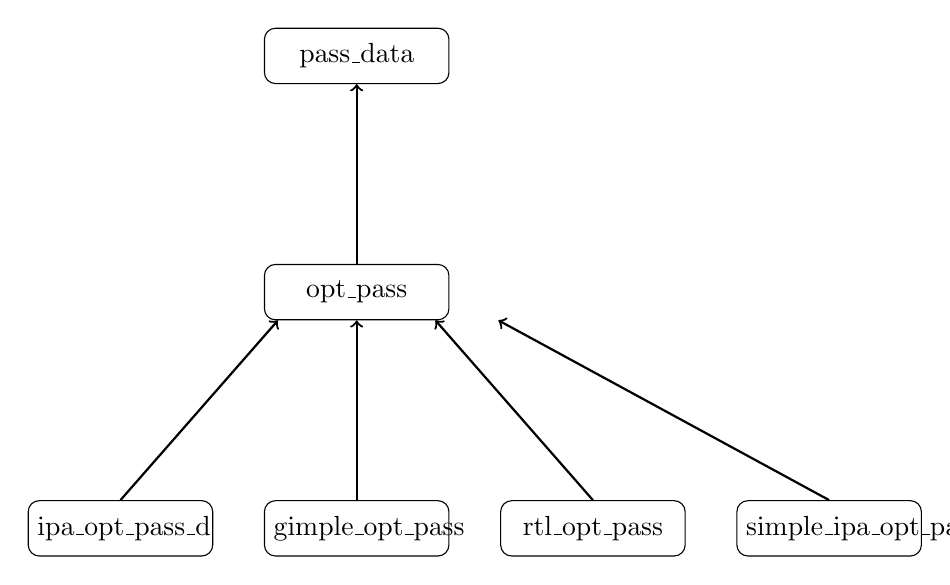
\begin{tikzpicture}[node distance = 5cm, auto]
    % Place nodes
    \node [block]                         (pass_data)   {pass\_data};
    \node [block, below of=pass_data]     (opt_pass) {opt\_pass};

    \node [block, below of=opt_pass]        (gimple_opt_pass) {gimple\_opt\_pass};
    \node [block, left of=gimple_opt_pass] (ipa_opt_pass_d)  {ipa\_opt\_pass\_d};
    \node [block, right of=gimple_opt_pass]  (rtl_opt_pass)    {rtl\_opt\_pass};
    \node [block, right of=rtl_opt_pass]    (simple_ipa_opt_pass) {simple\_ipa\_opt\_pass};

    % Draw edges
    \draw[->, thick]    (opt_pass.north)          -- (pass_data.south);

    \draw[->, thick]    (gimple_opt_pass.north)      -- (opt_pass.south);
    \draw[->, thick]    (ipa_opt_pass_d.north)       -- ([xshift=-1cm]opt_pass.south);
    \draw[->, thick]    (rtl_opt_pass.north)         -- ([xshift=1cm]opt_pass.south);
    \draw[->, thick]    (simple_ipa_opt_pass.north)  -- ([xshift=1.8cm]opt_pass.south);


\end{tikzpicture}
%}
\end{center}
\caption{Hierarquia dos passos de otimização do GCC.}
\label{fig:opt_uml}
\end{figure}


\end{subsection}

%    Para realizar otimizações considerando as interações entre as rotinas,
%é utilizado um grafo de chamada de funções (\texttt{cgraphs}). Aqui as rotinas são
%representadas como um vértice no grafo, e existe um arco de $f$ à $g$
%quando há uma chamada de $g$ a partir de $f$. Dependendo da linguagem de
%programação utilizada, construir tais grafos pode ser uma tarefa simples pois
%as chamadas são especificadas estaticamente, como é o caso de Fortran; mas
%isto pode se tornar algo extremamente complexo quando orientação à objetos é
%empregada, pois é possível sobrescrever métodos.
%
%    Os grafos de chamadas de funções permitem otimizações que eliminem chamadas
%de funções, economizando assim o custo da chamada, e ainda permitem com que as
%funções sejam emitidas por ordem de proximidade, evitando com que o salto no
%fluxo de execução seja demasiado longo, o que implicaria em \textit{cache miss}.
%Também é possível propagar informações a respeito de outras funções, por exemplo
%propagar que uma certa função não altera um estado global ou interno desta
%(e.g. imprimir na tela, alterar um objeto), e em seguida calcular o resultado
%desta em tempo de compilação e remover sua chamada. Isto permite binários menores
%e código mais rápido, pois evita a necessidade de computar valores em tempo de
%execução.
%

%Um exemplo é o \textit{Register Transfer Language} (RTL) onde o código é
%representado como uma sequência de instruções em uma máquina de infinitos
%registradores. 

\begin{subsection}{GNU Toolchain e o Processo Clássico de Compilação}

    Um \textit{toolchain} é um conjunto de ferramentas que são ligadas em
cascata para o desenvolvimento de \textit{software}. Normalmente o
\textit{toolchain} consiste em um compilador, um montador e um linkeditor,
mas também pode conter mais ferramentas, como um \textit{debugger}.

A GNU providencia um conjunto de ferramentas para desenvolvimento de software
conhecido como GNU \textit{toolchain}. São parte desse toolchain:
\begin{itemize}
    \item \textit{Binutils}, um conjunto de ferramentas contendo o linkeditor
LD, o montador AS, e outras ferramentas\footnote{\url{https://www.gnu.org/software/binutils/}}.

    \item O driver \texttt{gcc}, responsável por chamar os compiladores \texttt{cc1},
        \texttt{cc1plus}, \texttt{f951} para C, C++ e Fortran, respectivamente,
        e também responsável por interagir com as demais ferramentas do 
        \textit{Toolchain}.

    \item A biblioteca \texttt{glibc}.

    \item O \textit{debugger} GDB.
\end{itemize}

As ferramentas acima interagem umas com as outras da seguinte forma: primeiro, o código na
Linguagem Fonte é compilado usando o GCC para a linguagem de máquina, em seguida, o código
é montado utilizando o AS (que constrói o arquivo objeto) e por fim o linkeditor
LD coleta todos os arquivos objetos gerados, construindo o binário especificado. A Figura
\ref{fig:gnu_toolchain} retrata esse processo.


\begin{figure}
\tikzstyle{block} = [rectangle, draw, fill=white,
    text width=6em, text centered, rounded corners, node distance=6.5cm, auto, minimum height=2em]
\tikzstyle{line} = [draw, -latex]
\tikzstyle{cloud} = [draw, ellipse,fill=white, node distance=2cm,
    minimum height=2em]
\begin{center}
\scalebox{0.7}{
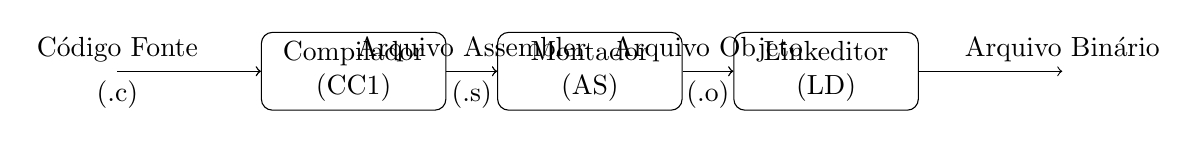
\begin{tikzpicture}[node distance = 3cm, auto]
    % Place nodes
    \node [block]                      (cc1) {Compilador \\ (CC1)};
    \node [block, right of = cc1]      (as) {Montador\\(AS)};
    \node [block, right of = as]       (ld) {Linkeditor\\(LD)};
    \coordinate [left of=cc1]          (fonte);
    \coordinate [right of=ld]    (bin);

    % Draw edges
    \draw[->]    (cc1.east)    -- (as.west)       node[midway, above] {Arquivo Assembler};
    \draw[->]    (cc1.east)    -- (as.west)       node[midway, below] {(.s)};
    \draw[->]    (as.east)     -- (ld.west)       node[midway, above] {Arquivo Objeto};
    \draw[->]    (as.east)     -- (ld.west)       node[midway, below] {(.o)};
    \draw[->]    (fonte.west)  -- (cc1.west)      node[pos=0, above] {Código Fonte};
    \draw[->]    (fonte.west)  -- (cc1.west)      node[pos=0, below] {(.c)};
    \draw[->]    (ld.east)     -- (bin.west)      node[pos=1, above] {Arquivo Binário};
\end{tikzpicture}
}
\end{center}
\caption{Etapas de compilação.}
\label{fig:gnu_toolchain}
\end{figure}

Esse processo é tradicionalmente usado para compilar \textit{softwares} complexos,
em conjunto com uma ferramenta que controla a geração de arquivos objetos e executáveis
como o GNU Make, como ilustrado na Figura \ref{fig:classical_build}. Aqui cada arquivo
é compilado individualmente, passando por todos os processos da compilação (tradução
para a linguagem intermediária, otimização, tradução para a Linguagem Alvo,
e encapsulamento no arquivo objeto), para que em seguida eles sejam ligados por um
linkeditor como o LD. Através do Make, onde é possível explicitar as dependências de
um arquivo, a compilação pode ser efeutada em paralelo entre arquivos que não dependem
uns dos outros.

Neste processo, não é possível aplicar otimizações observando o programa como
um todo, pois o compilador não tem informações sobre as funções que estão em
outros arquivos. Sendo assim, todas as otimizações são aplicadas localmente
usando apenas o contexto do arquivo.

\begin{figure}
\tikzstyle{block} = [rectangle, draw, fill=white,
    text width=6em, text centered, rounded corners, node distance=3cm, auto, minimum height=2em]
\tikzstyle{line} = [draw, -latex]
\tikzstyle{cloud} = [draw, ellipse,fill=white, node distance=2cm,
    minimum height=2em]
\begin{center}
\scalebox{0.7}{
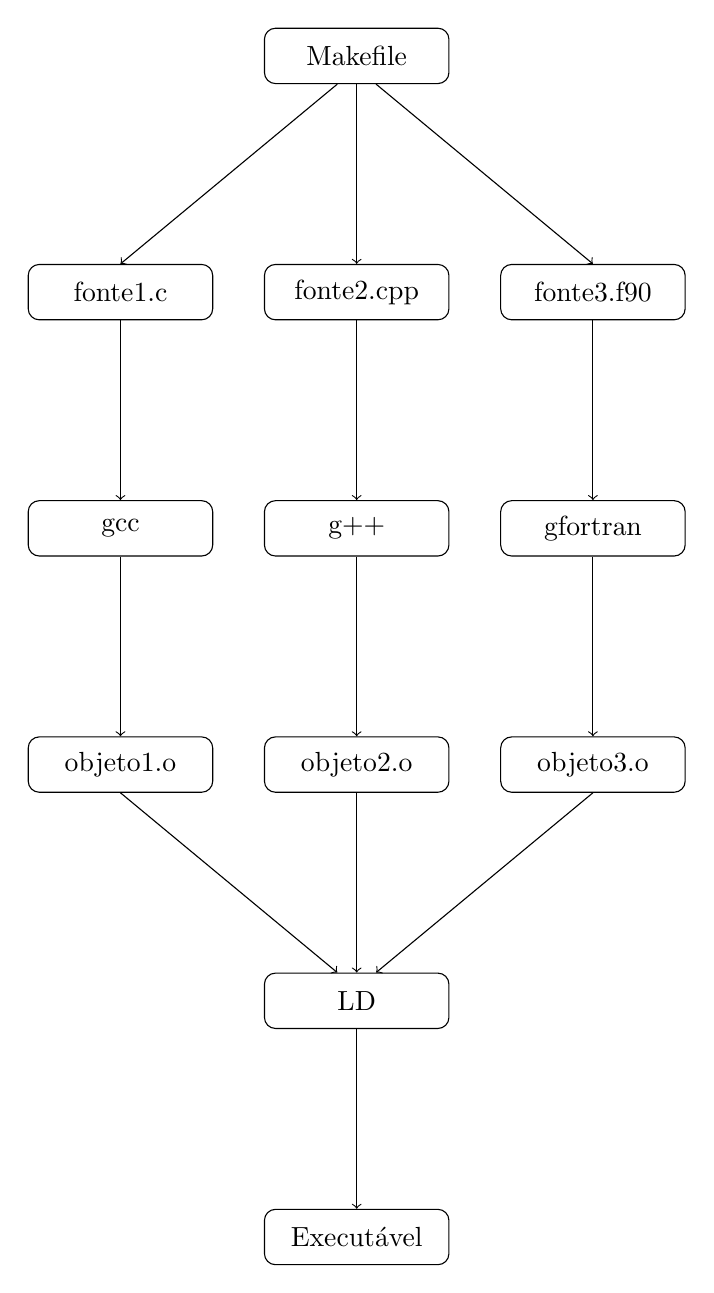
\begin{tikzpicture}[node distance = 3cm, auto]
    % Place nodes
    \node [block]                         (make)   {Makefile};
    \coordinate[below of=make]            (c);
    \node [block, left of=c]              (fonte1) {fonte1.c};
    \node [block, right of=fonte1]        (fonte2) {fonte2.cpp};
    \node [block, right of=fonte2]        (fonte3) {fonte3.f90};

    \node [block, below of=fonte1]        (gcc)      {gcc};
    \node [block, below of=fonte2]        (g++)      {g++};
    \node [block, below of=fonte3]        (gfortran) {gfortran};

    \node [block, below of=gcc]           (objeto1) {objeto1.o};
    \node [block, below of=g++]           (objeto2) {objeto2.o};
    \node [block, below of=gfortran]      (objeto3) {objeto3.o};

    \node [block, below of=objeto2]       (ld) {LD};

    \node [block, below of=ld]            (bin) {Executável};

    % Draw edges
    \draw[->]    ([xshift=-0.7em] make.south)   -- (fonte1.north);
    \draw[->]    (make.south)   -- (fonte2.north);
    \draw[->]    ([xshift=+0.7em] make.south)   -- (fonte3.north);

    \draw[->]    (fonte1.south)   -- (gcc.north);
    \draw[->]    (fonte2.south)   -- (g++.north);
    \draw[->]    (fonte3.south)   -- (gfortran.north);

    \draw[->]    (gcc.south)   -- (objeto1.north);
    \draw[->]    (g++.south)   -- (objeto2.north);
    \draw[->]    (gfortran.south)   -- (objeto3.north);

    \draw[->]    (objeto1.south)   -- ([xshift=-0.7em]ld.north);
    \draw[->]    (objeto2.south)   -- (ld.north);
    \draw[->]    (objeto3.south)   -- ([xshift=+0.7em]ld.north);

    \draw[->]    (ld.south)   -- (bin.north);


\end{tikzpicture}
}
\end{center}
\caption{Processo clássico de compilação de um programa.}
\label{fig:classical_build}
\end{figure}


\end{subsection}

\end{section}

\begin{section}{Computação Paralela}
\label{sec:parallel_comp}

    A Computação Paralela é o ato de coordenar vários fluxos de
execução operando simultaneamente em um ou mais computadores para
atingir um objetivo em comum. Ela se tornou uma tendência na
computação contemporânea por conta da facilidade de aquisição
e custo de produção reduzido dos processadores \textit{multicore}
e \textit{manycore}, em relação a um processador de igual desempenho
com apenas um núcleo.

    Para ilustrar a evolução dos processadores \textit{multicore}, \cite{42years}
    publicou um gráfico mostrando o número
de transistores, núcleos e desempenho de cada núcleo desde 1970,
apresentado na Figura \ref{fig:42years}.
Neste gráfico é possível notar que a Lei de Moore ainda se aplica,
mas a desempenho sequencial dos processadores está em desaceleração,
enquanto o número de núcleos cresce exponencialmente desde 2008. Isto
justifica o uso de computação paralela sempre que possível para que
seja utilizado o máximo dos recursos computacionais disponíveis.

    Nessa seção são discutidas alguns conceitos básicos de computação
paralela e alguns algoritmos úteis na paralelização de programas.

\begin{figure}[ht]
 \centering
 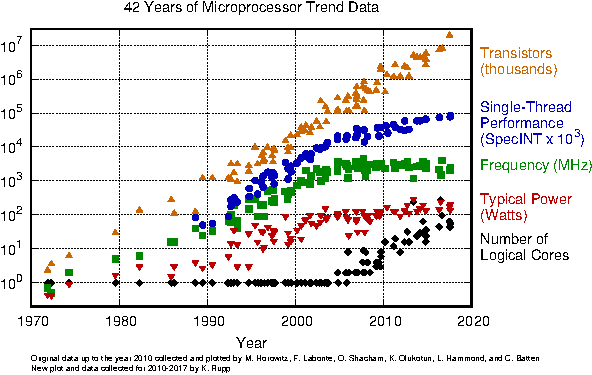
\includegraphics[scale=1.2]{42-years-processor-trend.pdf}
 \caption{42 anos de evolução dos processadores. Fonte: \cite{42years}}
 \label{fig:42years}
\end{figure}

\begin{subsection}{\textit{Speedup}}
    Uma maneira de medir o ganho de tempo em uma implementação paralela
de um algoritmo é através no conceito de \textit{speedup}. Sejam $T_1$
o tempo do algoritmo sequencial e $T_n$ o tempo desse algoritmo paralelizado
    com $n$ núcleos de processamento. Então o \textit{speedup} $S_n$
é dado por:
    $$ S_n = \frac{T_1}{T_n} $$

\end{subsection}


\begin{subsection}{A Taxonomia de Flynn}
	Mesmo com a evolução dos processadores \textit{multicore} e
\textit{manycore}, estas não são as únicas arquiteturas disponíveis para
realizar computação paralela. Michael J. Flynn \citep{pacheco:2011} definiu
uma taxonomia das arquiteturas, mas vale destaque para duas delas:
\begin{enumerate}
    \item \textbf{SIMD} - \textit{Single Instruction, Multiple Data}. Isso se refere
        a processadores vetoriais que permitem que uma operação seja executada simultâneamente em
        todos os elementos de um vetor simultâneamente. Alguns exemplos são as
        instruções SSE da Intel, e também as \textit{Graphics Processing Units} (GPU),
        embora essa última não seja considerada uma arquitetura puramente SIMD.

    \item \textbf{MIMD} - \textit{Multiple Instruction, Multiple Data}. Isso se refere
        aos sistemas \textit{multicore} independentes, capazes de executar tarefas
        de maneira assíncrona. Aqui estão localizados ambas as arquiteturas de memória
        compartilhada e memória distribuída.
\end{enumerate}
\end{subsection}

\begin{subsection}{Programação Paralela em Memória Compartilhada}
	Uma maneira de permitir Computação Paralela é através de
uma memória compartilhada. Aqui vários processadores ou núcleos
são ligados através de um barramento a uma memória compartilhada entre
todos os processadores, que permite leitura e escrita de dados.
Para evitar problemas de concorrência, são necessários mecanismos de
travas e sincronização.

	 Aqui, muitos dos recursos para sincronização são fornecidos pelo
Sistema Operacional (OS), e portanto é necessário explicar um pouco
das abstrações que ele fornece.

\begin{subsubsection}{Processos e \textit{Threads}}

	Antigamente, os processadores eram capazes de executar apenas
um programa por vez. Com isto em mente, os desenvolvedores
de Sistemas Operacionais criaram uma série de abstrações para que fosse
possível dar a ilusão ao usuário que vários programas estavam executando
ao mesmo tempo. Embora isso não seja mais um fato, já que hoje os processadores
são capazes de executar vários fluxos de execução simultaneamente, essa
é a principal motivação do conceito de Processos e \textit{Threads}.

	Um \textit{Processo} é um modelo de abstração do Sistema Operacional que
dá a um programa a ilusão de que ele tem o monopólio do processador
\citep{love:2005}. Cada processo tem a sua região de memória privada por
padrão, e para que processos possam compartilhar memória, isso deve ser 
explicitado no programa. Um exemplo onde isso pode ser feito é através das
chamadas \texttt{shmget} do extinto \texttt{System V}, mas cujo o Linux ainda
oferece suporte \citep{shmget}.

Cada processo contém pelo menos um fluxo de execução, e cada fluxo de
execução é chamado de \textit{thread}. Cada \textit{thread} dentro
de um processo compartilha memória com as demais \textit{threads}
do processo, facilitando assim o desenvolvimento de mecanismos de
comunicação através de uma memória compartilhada.

\end{subsubsection}

\begin{subsubsection}{Mecanismos de Sincronização}

	Seja através de auxílio do \textit{hardware}, ou com algoritmos
puramente implementados em \textit{software}, o Sistema Operacional
costuma fornecer mecanismos de sincronização para coordenar as várias
\textit{threads} de um processo, ou até mesmo vários processos.

    Um dos mecanismos mais famosos são os \textit{Semáforos}
\citep{dijkstra1965}. Um semáforo nada mais é que um contador que assume
valores não negativos com duas operações atômicas: \texttt{P} para
decrementá-lo, e \texttt{V} para incrementá-lo. Quando o semáforo atinge o
valor 0, a \textit{thread} que em sequência tentar decrementá-lo será bloqueada. A
sua execução apenas será retomada quando o semáforo for novamente incrementado
por outra \textit{thread} \citep{semaphore}.

    Semáforos também podem ser utilizados para resolver o problema da
seção crítica, que é uma seção de código que apenas uma \textit{thread}
deve poder executar por vez, embora seja mais comum a utilização
de \textit{Mutexes}.

\textit{Mutexes} nada mais são que uma estrutura que garante a exclusão
mútua de uma região, conforme ilustrado na Figura \ref{fig:mutex}. Nessa
figura, três \textit{threads} são iniciadas executando a função $f$, mas
apenas uma pode executar a seção crítica.
    Quando o \textit{mutex} \texttt{lock} é travado,
todas as outras \textit{threads} que tentarem acessar a seção crítica
serão bloqueadas pelo Sistema Operacional, garantindo assim que apenas
uma \textit{thread} esteja executando a seção crítica.
As \textit{threads} bloqueadas somente voltarão a executar quando o
    \textit{mutex} for desbloqueado pela \textit{thread} que o travou.
\begin{figure}
      \begin{lstlisting}[
        language=pseudocode,
        style=pseudocode,
        style=wider,
        functions={},
        specialidentifiers={extern, call, async, mutex_t},
      ]
        extern function mutex_lock, mutex_unlock;
        mutex_t lock;

        async function f()
            mutex_lock(lock);
                // Região crítica
            mutex_unlock(lock);
        end

        function main()
            for i=1, 3 do
                call f;
            done
        end
      \end{lstlisting}
      \caption{Ilustração de uso de um mutex,}
      \label{fig:mutex}
\end{figure}

Outro mecanismo de sincronização muito útil são as Barreiras. Uma barreira
é um ponto no programa onde, assim que a \textit{thread} o executar, ela
será bloqueada até que todas as \textit{threads} cheguem ao mesmo ponto, como
ilustrado na Figura \ref{fig:barrier}.
Isso é bastante útil para evitar que uma \textit{thread} avance na execução
do código enquanto ela deveria estar aguardando o resultado da computação
de outras \textit{threads}. As barrerias também costumam receber um parâmetro
de inicialização indicando quantas \textit{threads} precisam atingir a
barreira para que todas as \textit{threads} que a atingiu sejam desbloqueadas.

\begin{figure}[ht]
 \centering
 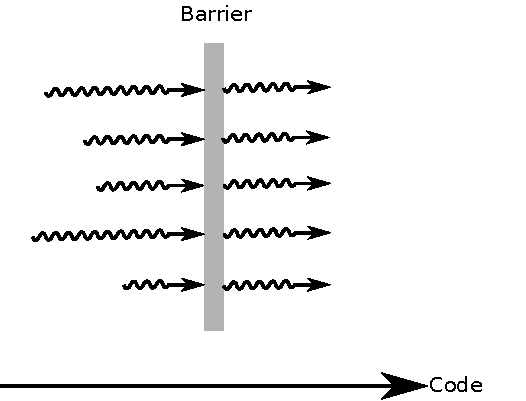
\includegraphics[scale=1.0]{barrier.pdf}
 \caption{Ilustração do funcionamento de uma barreira.}
 \label{fig:barrier}
\end{figure}


Por fim, exceto os semáforos, todos esses mecanismos mencionados acima são
implementados na biblioteca \texttt{Pthread}. Já os semáforos estão disponíveis
no Linux através da interface \texttt{semaphore.h}.

\end{subsubsection}

%\begin{subsubsection}{O Problema do Produtor-Consumidor}
%    Uma estrutura de dados muito útil em computação paralela
%é uma fila completamente \textit{Thread-safe}, ou seja,
%que várias \textit{threads} possam inserir e remover dados dessa
%fila simultaneamente sem o risco de perda de dados. Essa fila
%pode ser usada na comunicação entre as \textit{threads}, por
%exemplo: uma insere trabalho na fila, outra retira trabalho da
%fila. Isso permite com que \textit{pipelines}, ou escalonamento
%dinâmico de trabalho sejam implementados.
%
%Para implementar essa fila, são necessários dois semáforos e um
%\textit{mutex}. Um semáforo deve ser inicializado com o tamanho máximo
%da fila, e na inserção de um dado, esse semáforo deve ser decrementado
%para que, quando a fila estiver cheia, as \textit{threads} que tentarem
%inserir nela sejam bloqueadas. O outro semáforo deve ser iniciado com
%0, indicando que a fila está vazia, e incrementado quando um item for
%inserido na fila. Esse semáforo tem a finalidade de
%bloquear as \textit{threads} que tentarem remover elementos dessa
%fila quando ela estiver vazia. Assim que dados forem inseridos ou removidos
%da fila, as \textit{threads} são devidamente ``despertadas''. Isso evita gasto
%desnecessário de ciclos de processamento por não utilizar uma técnica
%chamada \textit{espera ocupada}. Por fim, um \textit{Mutex} deve ser
%utilizado para evitar problemas de concorrência ao incrementar e
%decrementar os apontadores de inicio e fim da fila.
%Uma implementação
%é apresentada na Figura \ref{fig:prod_consumer}.
%\begin{figure}
%      \begin{lstlisting}[
%        language=pseudocode,
%        style=pseudocode,
%        style=wider,
%        functions={},
%        specialidentifiers={extern, call, async, int, class, mod, semaphore_t, mutex_t},
%      ]
%        class Fifo
%            int buffer[];
%            int size;
%            int head, tail;
%            semaphore_t full, empty;
%            mutex_t lock
%
%            function init(n)
%                buffer = allocate_memory(n);
%                head, tail = 0;
%                sem_init(empty, n);
%                sem_init(full, 0);
%                mutex_init(lock);
%                size = n;
%            end
%
%            function push(element)
%                sem_p(empty);
%                mutex_lock(lock);
%                buffer[head] = element;
%                head = head + 1 mod size;
%                mutex_unlock(lock);
%                sem_v(full);
%            end
%
%            function pop()
%                sem_p(full);
%                mutex_lock(lock);
%                ret = buffer[tail];
%                tail = tail + 1 mod size;
%                mutex_unlock(lock);
%                sem_v(empty)
%
%                return ret;
%            end
%        end 
%
%      \end{lstlisting}
%      \caption{Uma implementação do Produtor-Consumidor.}
%      \label{fig:prod_consumer}
%\end{figure}
%
%\end{subsubsection}

\end{subsection}

\end{section}
